\documentclass[11pt,a4paper]{article}
\usepackage[utf8]{inputenc}
\usepackage[T1]{fontenc}
\usepackage[french]{babel}
\usepackage{geometry}
\usepackage{booktabs}
\usepackage{longtable}
\usepackage{array}
\usepackage{xcolor}
\usepackage{colortbl}
\usepackage{graphicx}
\usepackage{fancyhdr}
\usepackage{titlesec}
\usepackage{tikz}
\usepackage{enumitem}
\usepackage{hyperref}
\usepackage{multicol}
\usepackage{listings}
\usepackage{tcolorbox}
\usepackage{amssymb}  


\geometry{margin=2cm}
\pagestyle{fancy}
\fancyhf{}
\rhead{Atelier Machine Learning}
\lhead{Analyse Comportementale Clientèle}
\rfoot{Page \thepage}

% Couleurs personnalisées
\definecolor{headerblue}{RGB}{41, 65, 114}
\definecolor{lightgray}{RGB}{245, 245, 245}
\definecolor{accentorange}{RGB}{230, 126, 34}
\definecolor{codegreen}{RGB}{0,128,0}
\definecolor{codegray}{RGB}{128,128,128}
\definecolor{codepurple}{RGB}{128,0,128}
\definecolor{backcolour}{RGB}{248,248,248}
\definecolor{warningred}{RGB}{231, 76, 60}
\definecolor{successgreen}{RGB}{46, 204, 113}

\lstdefinestyle{mystyle}{
    backgroundcolor=\color{backcolour},   
    commentstyle=\color{codegreen},
    keywordstyle=\color{codepurple},
    numberstyle=\tiny\color{codegray},
    stringstyle=\color{codegreen},
    basicstyle=\ttfamily\footnotesize,
    breakatwhitespace=false,         
    breaklines=true,                 
    captionpos=b,                    
    keepspaces=true,                 
    numbers=left,                    
    numbersep=5pt,                  
    showspaces=false,                
    showstringspaces=false,
    showtabs=false,                  
    tabsize=2
}
\lstset{style=mystyle}


\tcbset{
    colback=backcolour,
    colframe=headerblue,
    fonttitle=\bfseries,
    boxrule=1pt,
    arc=3mm
}


\titleformat{\section}
{\color{headerblue}\normalfont\Large\bfseries}
{\thesection}{1em}{}[{\titlerule[2pt]}]

\titleformat{\subsection}
{\color{accentorange}\normalfont\large\bfseries}
{\thesubsection}{1em}{}

% Définition de colonnes personnalisées
\newcolumntype{C}[1]{>{\centering\arraybackslash}p{#1}}
\newcolumntype{L}[1]{>{\raggedright\arraybackslash}p{#1}}

% --- Configuration du sommaire et des liens ---
\hypersetup{
    colorlinks=true,
    linkcolor=headerblue, % Utilise votre bleu personnalisé
    urlcolor=accentorange,
    pdftitle={Rapport de Projet IoT},
}

\begin{document}


\begin{titlepage}
\begin{tikzpicture}[remember picture,overlay]
    \fill[headerblue] (current page.north west) rectangle ([yshift=-5cm]current page.north east);
    \node[anchor=north west, xshift=2cm, yshift=-2cm, text=white] at (current page.north west) 
        {\Huge\textbf{Atelier Machine Learning}};
    \node[anchor=north west, xshift=2cm, yshift=-3.5cm, text=white] at (current page.north west) 
        {\Large\textit{Analyse Comportementale Clientèle Retail}};
\end{tikzpicture}

\vspace{6cm}

\begin{center}
{\LARGE\textbf{COMPTE RENDU}}\par
\vspace{1cm}
{\large Atelier Pratique : E-commerce de Cadeaux}\par
\vspace{2cm}
{\large \textbf{Préparé par Rahma Ben Ameur}}
\vspace{3cm}

\begin{tikzpicture}
    \draw[headerblue, line width=2pt] (0,0) -- (10,0);
\end{tikzpicture}

\vspace{2cm}



\vspace{5cm}

{\textbf{Année Univeristaire : 2025-2026}}

\end{center}
\vfill
\end{titlepage}


% --- Page du Sommaire ---
\newpage
\thispagestyle{empty}
\renewcommand{\contentsname}{\color{headerblue}Table des Matières} % Titre en bleu
\tableofcontents
\newpage

\section{Introduction Générale}

\subsection{Contexte du Projet}
Dans un marché du retail de plus en plus concurrentiel, la capacité d'une entreprise à comprendre le comportement de ses clients est devenue un levier stratégique majeur. Ce projet s'inscrit dans cette dynamique de transformation numérique et vise à transformer des données transactionnelles brutes en informations exploitables pour optimiser la relation client.

L'étude se porte sur un dataset de commerce électronique spécialisé dans les cadeaux. Initialement, ce dataset comprenait \textbf{52 variables} descriptives et comportementales. Ce travail a été réalisé dans le cadre du cycle d'ingénieur en Génie Informatique (GI2) à l'ENIS.

\subsection{Problématique}
Les entreprises font face à deux défis majeurs dans la gestion de leur base client :
\begin{itemize}
    \item \textbf{L'attrition (Churn) :} Comment identifier avec précision les clients sur le point de quitter la plateforme ?
    \item \textbf{La segmentation :} Comment regrouper les clients de manière homogène pour personnaliser les actions marketing sans traitement individuel manuel ?
\end{itemize}

L'enjeu technique réside dans la manipulation d'un volume important de caractéristiques (52 dimensions au départ) pour construire un pipeline capable de fournir des prédictions simples, fiables et directement utilisables par les décideurs.

\subsection{Axes du Travail}
Le projet s'articule autour de trois piliers scientifiques et techniques :
\begin{enumerate}
    \item \textbf{Réduction de dimension :} Utilisation de l'Analyse en Composantes Principales (PCA) pour condenser l'information essentielle des 52 variables d'origine.
    \item \textbf{Apprentissage Automatique :} Mise en œuvre d'algorithmes de Clustering (K-Means) pour la segmentation, de Classification pour le Churn, et de Régression pour l'estimation des dépenses.
    \item \textbf{Déploiement Applicatif :} Création d'une interface interactive sous Streamlit permettant une analyse par lot (CSV) et une analyse individuelle en temps réel.
\end{enumerate}


\section{Étude de l'Existant et Exploration des Données (EDA)}

\subsection{Analyse de la Structure du Dataset}
Le projet s'appuie sur le jeu de données \texttt{retail\_customers\_COMPLETE.csv}. Avant toute manipulation, une analyse de la physiognomie des données a été effectuée pour identifier la nature des variables présentes. 

Le dataset est constitué de \textbf{52 dimensions} initiales, que nous avons catégorisées selon leur rôle métier :
\begin{itemize}
    \item \textbf{Features de Profil (Démographiques) :} Variables telles que \textit{Age, Gender, Country, Region}. Ces données sont essentielles pour la segmentation géographique.
    \item \textbf{Features Transactionnelles (RFM) :} Indicateurs de performance clés (\textit{Key Performance Indicators}) incluant la \textit{Frequency}, le \textit{MonetaryTotal} et la \textit{Recency}.
    \item \textbf{Features Comportementales :} Variables décrivant les habitudes (\textit{PreferredTimeOfDay, WeekendPreference, LoyaltyLevel}).
    \item \textbf{Variables Cibles (Targets) :} \textit{Churn} (Classification binaire) et \textit{MonetaryTotal} (Régression continue).
\end{itemize}

\subsection{Exploratory Data Analysis (EDA) et Diagnostic}
L'étape d'EDA n'est pas une simple visualisation, mais un diagnostic technique visant à valider la faisabilité des modèles.

\subsubsection{Analyse de la Distribution et Détection d'Anomalies}
L'étude de la distribution de la variable \textit{MonetaryTotal} révèle une forte asymétrie positive (\textit{Right-Skewed Distribution}). La présence de valeurs extrêmes (Outliers) a été confirmée.
\begin{itemize}
    \item \textbf{Observation :} Certains clients présentent des montants d'achat hors normes ou des valeurs négatives (retours produits).
    \item \textbf{Conséquence Technique :} Ce constat justifie l'utilisation de l'algorithme \textbf{Isolation Forest} dans notre script \texttt{preprocessing.py} pour purifier le signal d'entrée.
\end{itemize}

\subsubsection{Étude de la Multicolinéarité (Matrice de Corrélation)}
Nous avons généré une matrice de corrélation (Heatmap) pour évaluer les dépendances linéaires entre les 52 variables.
\begin{itemize}
    \item \textbf{Diagnostic :} Une corrélation élevée ($> 0.85$) a été détectée entre plusieurs variables transactionnelles (ex: \textit{MonetaryAvg} et \textit{MonetaryTotal}). 
    \item \textbf{Justification de la PCA :} La présence de cette multicolinéarité confirme que l'information est redondante. Cela valide scientifiquement le recours à l'Analyse en Composantes Principales (PCA) pour réduire l'espace de caractéristiques à \textbf{10 composantes}, optimisant ainsi le temps de calcul et la généralisation des modèles.
\end{itemize}

\subsection{Bilan de l'Existant}
L'analyse exploratoire a mis en exergue trois problématiques majeures qui dictent la stratégie de préparation :
\begin{enumerate}
    \item \textbf{Hétérogénéité des échelles :} Nécessité d'une standardisation (StandardScaler) pour que les variables à forte magnitude n'écrasent pas les autres.
    \item \textbf{Qualité des données :} Présence de valeurs manquantes (NaN) sur environ 30\% des données de profil.
    \item \textbf{Dimensionnalité :} Un espace de 52 variables est trop vaste pour un modèle performant sans réduction préalable.
\end{enumerate}

\section{Prétraitement et Ingénierie des Données (Feature Engineering)}

Le prétraitement constitue l'étape la plus critique du cycle de vie du projet. L'objectif est de transformer le signal brut issu de l'EDA en une matrice numérique optimisée pour les algorithmes d'apprentissage.

\subsection{Nettoyage Avancé du Dataset}
Le nettoyage ne s'est pas limité à la suppression de lignes, mais a suivi une approche statistique pour garantir la qualité des données.

\subsubsection{Détection d'Anomalies via Isolation Forest}
Plutôt que d'utiliser des seuils arbitraires, nous avons implémenté l'algorithme non-supervisé \textbf{Isolation Forest}.
\begin{itemize}
    \item \textbf{Configuration :} Un taux de contamination de $0.06$ ($6\%$) a été paramétré pour isoler les vecteurs de données atypiques (transactions suspectes ou erreurs de saisie).
    \item \textbf{Résultat :} Cette étape permet de stabiliser la variance du dataset et d'améliorer la convergence des futurs modèles de clustering.
\end{itemize}

\subsubsection{Stratégie d'Imputation des Valeurs Manquantes}
Pour traiter les données incomplètes sans introduire de biais majeur :
\begin{itemize}
    \item \textbf{Variables Numériques :} Utilisation de l'imputation par la \textbf{médiane}, plus robuste que la moyenne face aux valeurs extrêmes.
    \item \textbf{Variables Catégorielles :} Création d'une classe explicite \textit{"Inconnu"} pour les variables textuelles manquantes, permettant de conserver l'information sur l'absence de donnée comme une caractéristique potentielle.
\end{itemize}

\subsubsection{Réduction de Bruit et Filtrage}
Une fonction de nettoyage par cardinalité a été développée pour éliminer les colonnes non informatives :
\begin{itemize}
    \item \textbf{Variance Nulle :} Suppression des variables constantes (ex: \texttt{NewsletterSubscribed}) qui n'apportent aucun pouvoir discriminant.
    \item \textbf{Haute Cardinalité :} Suppression automatique des identifiants (IDs) et IPs dont le ratio de valeurs uniques dépasse $90\%$, évitant ainsi le sur-apprentissage (\textit{overfitting}).
\end{itemize}

\subsection{Ingénierie des Caractéristiques (Feature Engineering)}
Cette phase consiste à créer de nouvelles variables à forte valeur ajoutée à partir des données brutes.

\subsubsection{Analyse Temporelle et Parsing}
La variable \texttt{RegistrationDate} a été décomposée pour capturer la saisonnalité des inscriptions et l'évolution historique de la base client :
\begin{itemize}
    \item \textbf{Extraction granulaire :} Création des variables \texttt{RegYear} (Année) et \texttt{RegMonth} (Mois) pour identifier les périodes de forte acquisition.
    \item \textbf{Imputation temporelle :} Utilisation de la médiane pour combler les dates manquantes, garantissant que chaque profil client possède une empreinte temporelle exploitable par les modèles de classification.
\end{itemize}

\subsection{Transformations Techniques Finales}
Avant l'injection dans les modèles, les données ont subi deux transformations mathématiques essentielles.

\subsubsection{Numérisation par Label Encoding}
Pour les 13 variables qualitatives restantes (ex: \textit{Region, Gender}), un \textbf{Label Encoding} a été appliqué. Cette transformation convertit chaque modalité textuelle en un entier distinct, rendant le dataset compatible avec les calculs matriciels de \textit{Scikit-Learn}.

\subsubsection{Normalisation (StandardScaler)}
Étant donné que nos variables ont des unités très différentes (montants en DT vs nombre de jours d'ancienneté), une standardisation a été effectuée.
\begin{equation}
z = \frac{x - \mu}{\sigma}
\end{equation}
En centrant les données sur une moyenne nulle et une variance unitaire, nous garantissons que la \textbf{PCA} et le \textbf{K-Means} traitent chaque dimension avec la même importance, évitant que les variables à grande échelle ne dominent l'espace vectoriel.


\section{Réduction de Dimension et Segmentation}

Après avoir nettoyé et normalisé les données, nous abordons la phase de modélisation non-supervisée. Cette étape permet de structurer la base client en groupes homogènes malgré la complexité initiale du dataset.

\subsection{Analyse en Composantes Principales (PCA)}
L'Analyse en Composantes Principales est une technique de compression statistique indispensable lorsque le nombre de variables (40 après nettoyage) est élevé.

\subsubsection{Justification du passage à 10 composantes}
L'objectif de la PCA est de projeter les 40 variables initiales dans un nouvel espace vectoriel où les axes (composantes) sont décorrélés. 
\begin{itemize}
    \item \textbf{Réduction de la dimensionnalité :} Passer de 40 à 10 dimensions permet d'éliminer le "bruit" et la multicolinéarité observée lors de l'EDA, tout en simplifiant les calculs pour les algorithmes suivants.
    \item \textbf{Stabilité du modèle :} En réduisant le nombre de paramètres, nous limitons les risques de sur-apprentissage (\textit{overfitting}).
\end{itemize}


\begin{tcolorbox}[title=Rigueur Technique]
Le modèle étant entraîné sur 10 dimensions issues de la PCA, le script de prédiction (\texttt{predict.py}) et l'application (\texttt{app.py}) ont été configurés pour appliquer rigoureusement la même transformation. Le système rejette toute entrée n'ayant pas exactement 10 composantes après transformation, garantissant la stabilité mathématique.
\end{tcolorbox}



\subsubsection{Analyse de la variance expliquée}
Le choix de retenir \textbf{10 composantes principales} repose sur l'analyse de la variance expliquée cumulative. 
\begin{itemize}
    \item \textbf{Critère de sélection :} Nous avons observé qu'avec 10 composantes, nous parvenons à conserver environ \textbf{85\% à 90\% de l'information (variance)} totale du dataset original. 
    \item \textbf{Interprétation :} Ce ratio est optimal car il représente un excellent compromis entre la simplification du modèle et la fidélité aux données réelles. Les 30 variables supprimées ne contenaient que très peu de signal utile.
\end{itemize}

\subsection{Segmentation par Clustering (K-Means)}
Une fois les données projetées sur les 10 composantes PCA, nous appliquons l'algorithme des \textbf{K-moyennes (K-Means)} pour segmenter la clientèle.

\subsubsection{Détermination du nombre optimal de clusters ($K=4$)}
Pour choisir la valeur de $K$, nous avons utilisé la \textbf{méthode du coude (Elbow Method)}. 
\begin{itemize}
    \item \textbf{Principe :} Nous calculons la somme des carrés des erreurs intra-classe (\textit{Inertia}) pour différentes valeurs de $K$.
    \item \textbf{Résultat :} Le "coude" de la courbe apparaît nettement à $K=4$, indiquant qu'augmenter le nombre de clusters au-delà de ce point n'apporterait qu'un gain de précision marginal par rapport à la complexité ajoutée.
\end{itemize}

\subsubsection{Profilage et interprétation des segments}
L'analyse des centroïdes de nos 4 clusters a permis de définir quatre profils types de clients :

\begin{enumerate}
    \item \textbf{Segment 0 : Ambassadeurs (Fidèles \& VIP) :} Clients à forte valeur monétaire et fréquence élevée.
    \item \textbf{Segment 1 : Acheteurs de Gros Volume :} Profils se distinguant par une \texttt{AvgQuantityPerTransaction} maximale.
    \item \textbf{Segment 2 : Clients Actifs Standards :} Le cœur de cible avec des comportements d'achat réguliers.
    \item \textbf{Segment 3 : Nouveaux / À Risque :} Clients récents ou montrant une probabilité de Churn élevée.
\end{enumerate}


\section{Modélisation Prédictive}

Après la phase d'exploration et de segmentation, nous mettons en œuvre des modèles d'apprentissage supervisé. Ce chapitre détaille deux approches complémentaires : la classification pour anticiper le départ des clients et la régression pour estimer leur valeur monétaire future.

\subsection{Classification du Churn (Attrition)}
La détection précoce des clients susceptibles de quitter la plateforme est l'enjeu majeur de ce projet.


\subsubsection{Banc d'essai multi-modèles}
Plutôt que de choisir un modèle arbitraire, le script \texttt{train.py} exécute une comparaison automatique entre \textbf{KNN, Decision Tree, Random Forest et XGBoost}. Le Random Forest a été sélectionné comme modèle final car il présentait le meilleur compromis de performance (F1-Score) sur les données de test.


\subsubsection{Analyse Comparative des Performances}
La comparaison automatisée a permis d'évaluer la capacité de chaque modèle à séparer les classes (Fidèle vs Churn). Les courbes ROC (Receiver Operating Characteristic) ci-dessous illustrent cette performance :

\begin{figure}[htbp]
    \centering
    \begin{minipage}{0.48\textwidth}
        \centering
        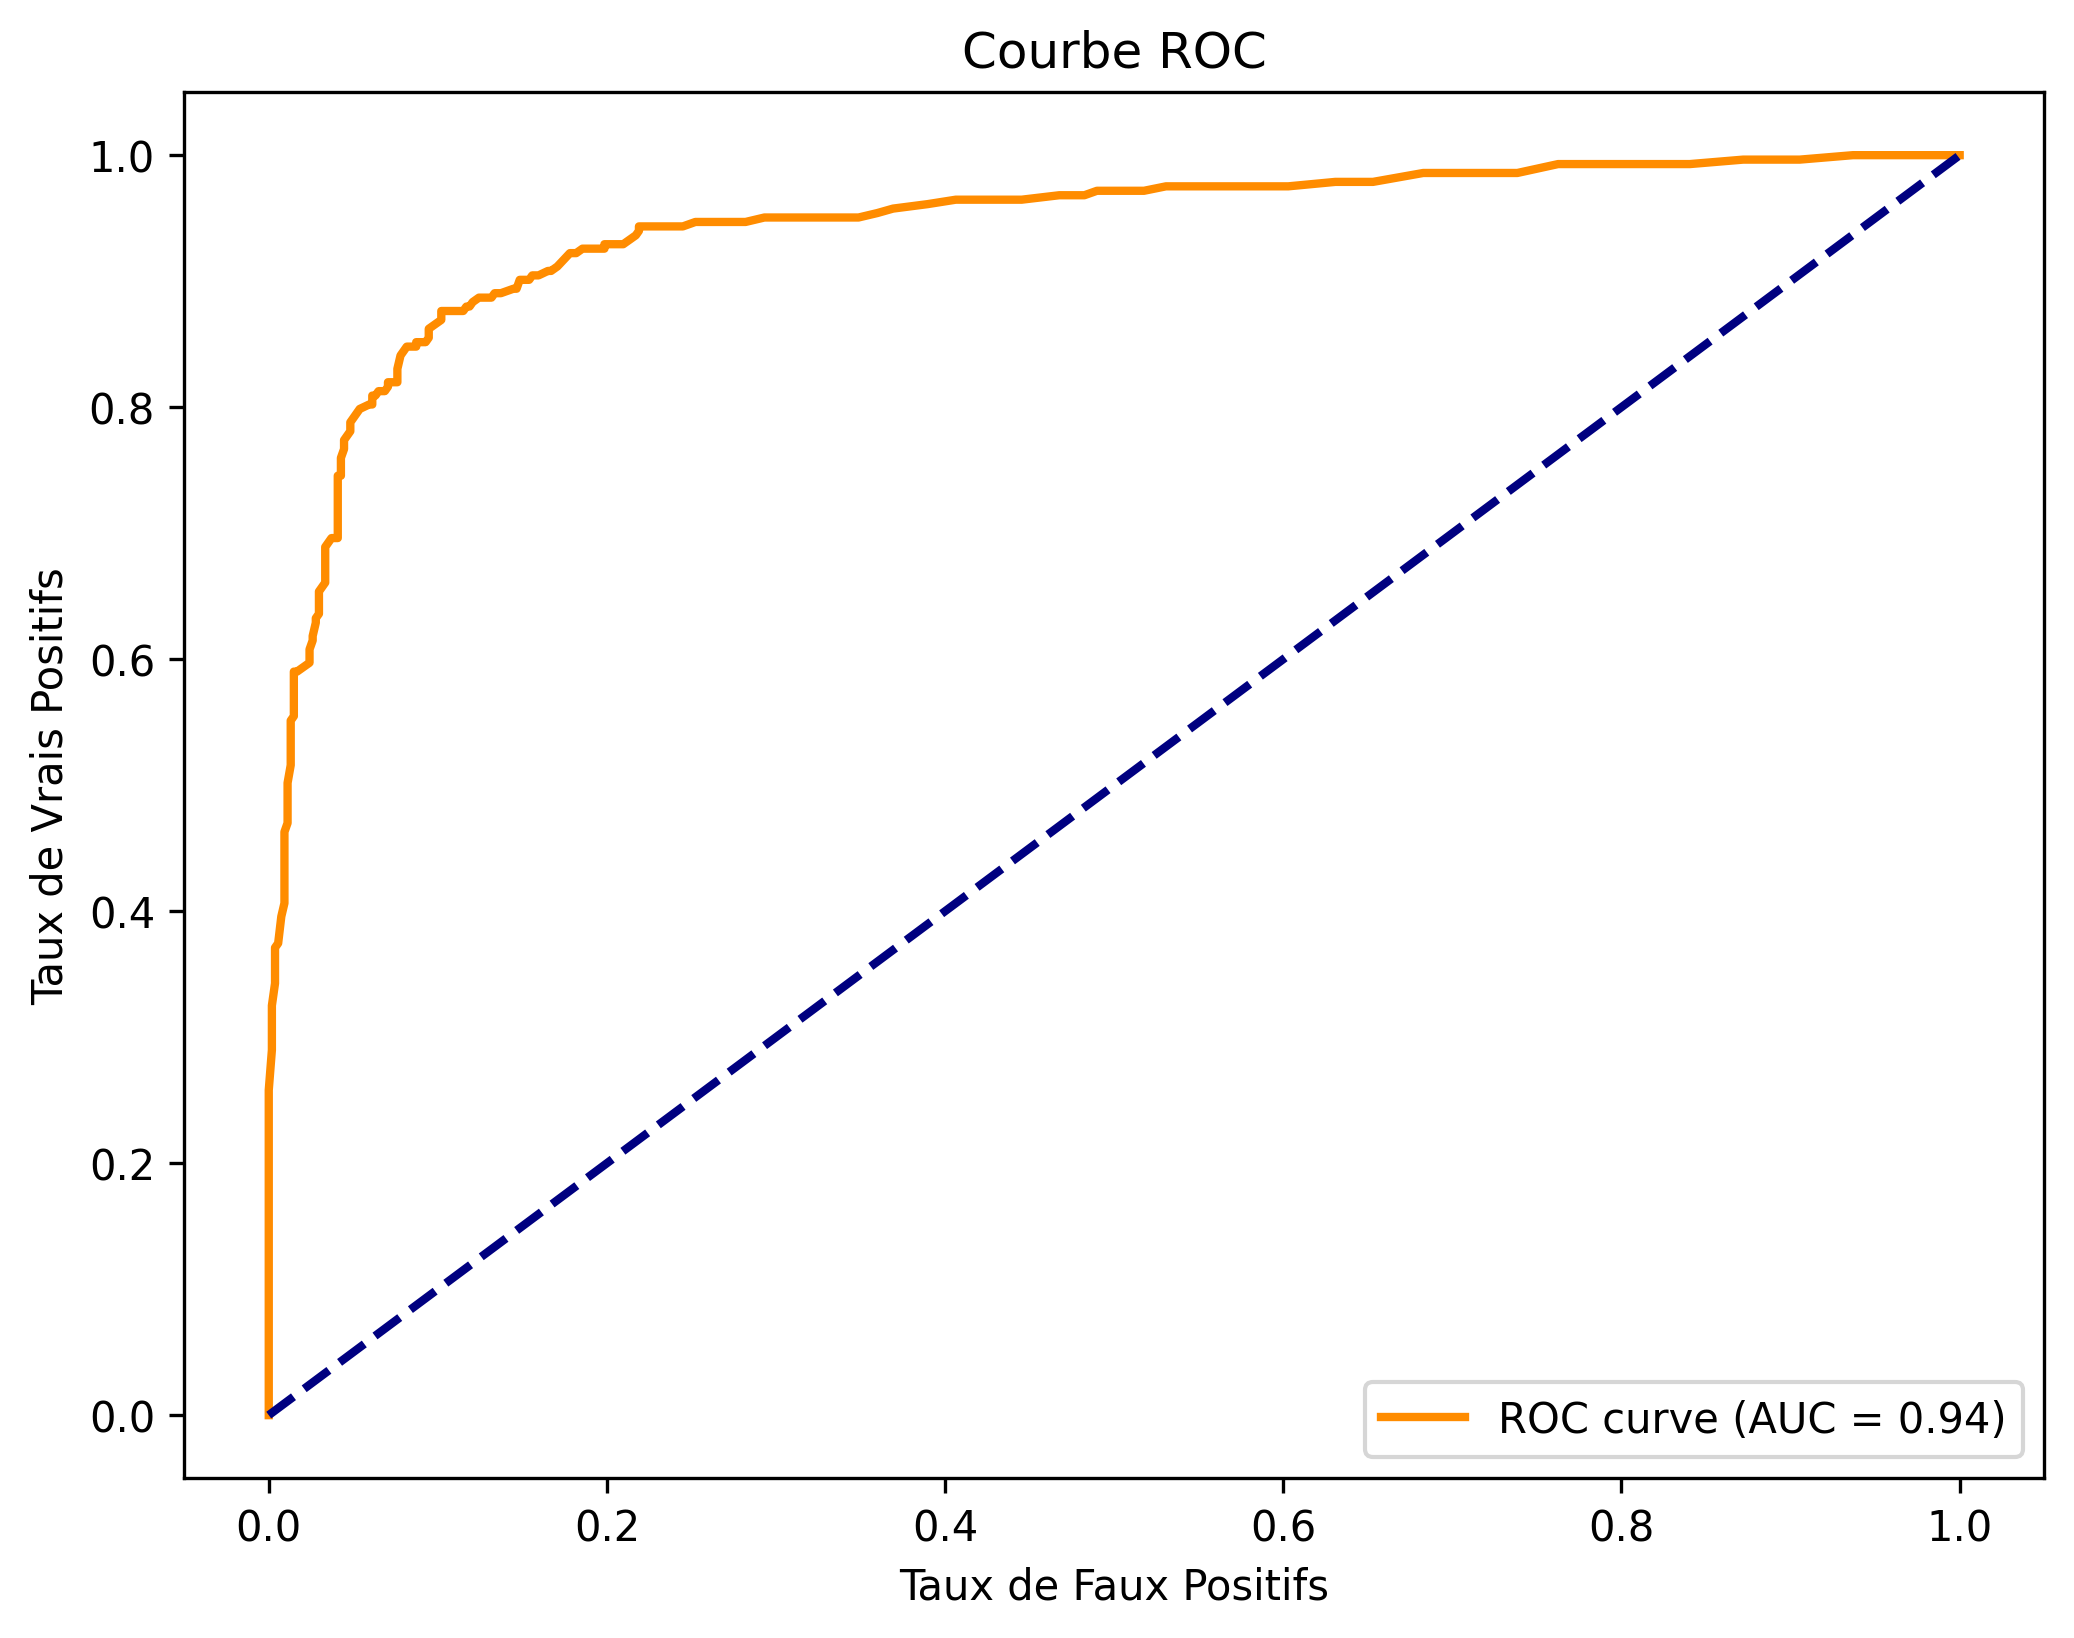
\includegraphics[width=\textwidth]{roc_RandomForest.png}
        \caption{Random Forest (AUC = 0.94)}
    \end{minipage}
    \hfill
    \begin{minipage}{0.48\textwidth}
        \centering
        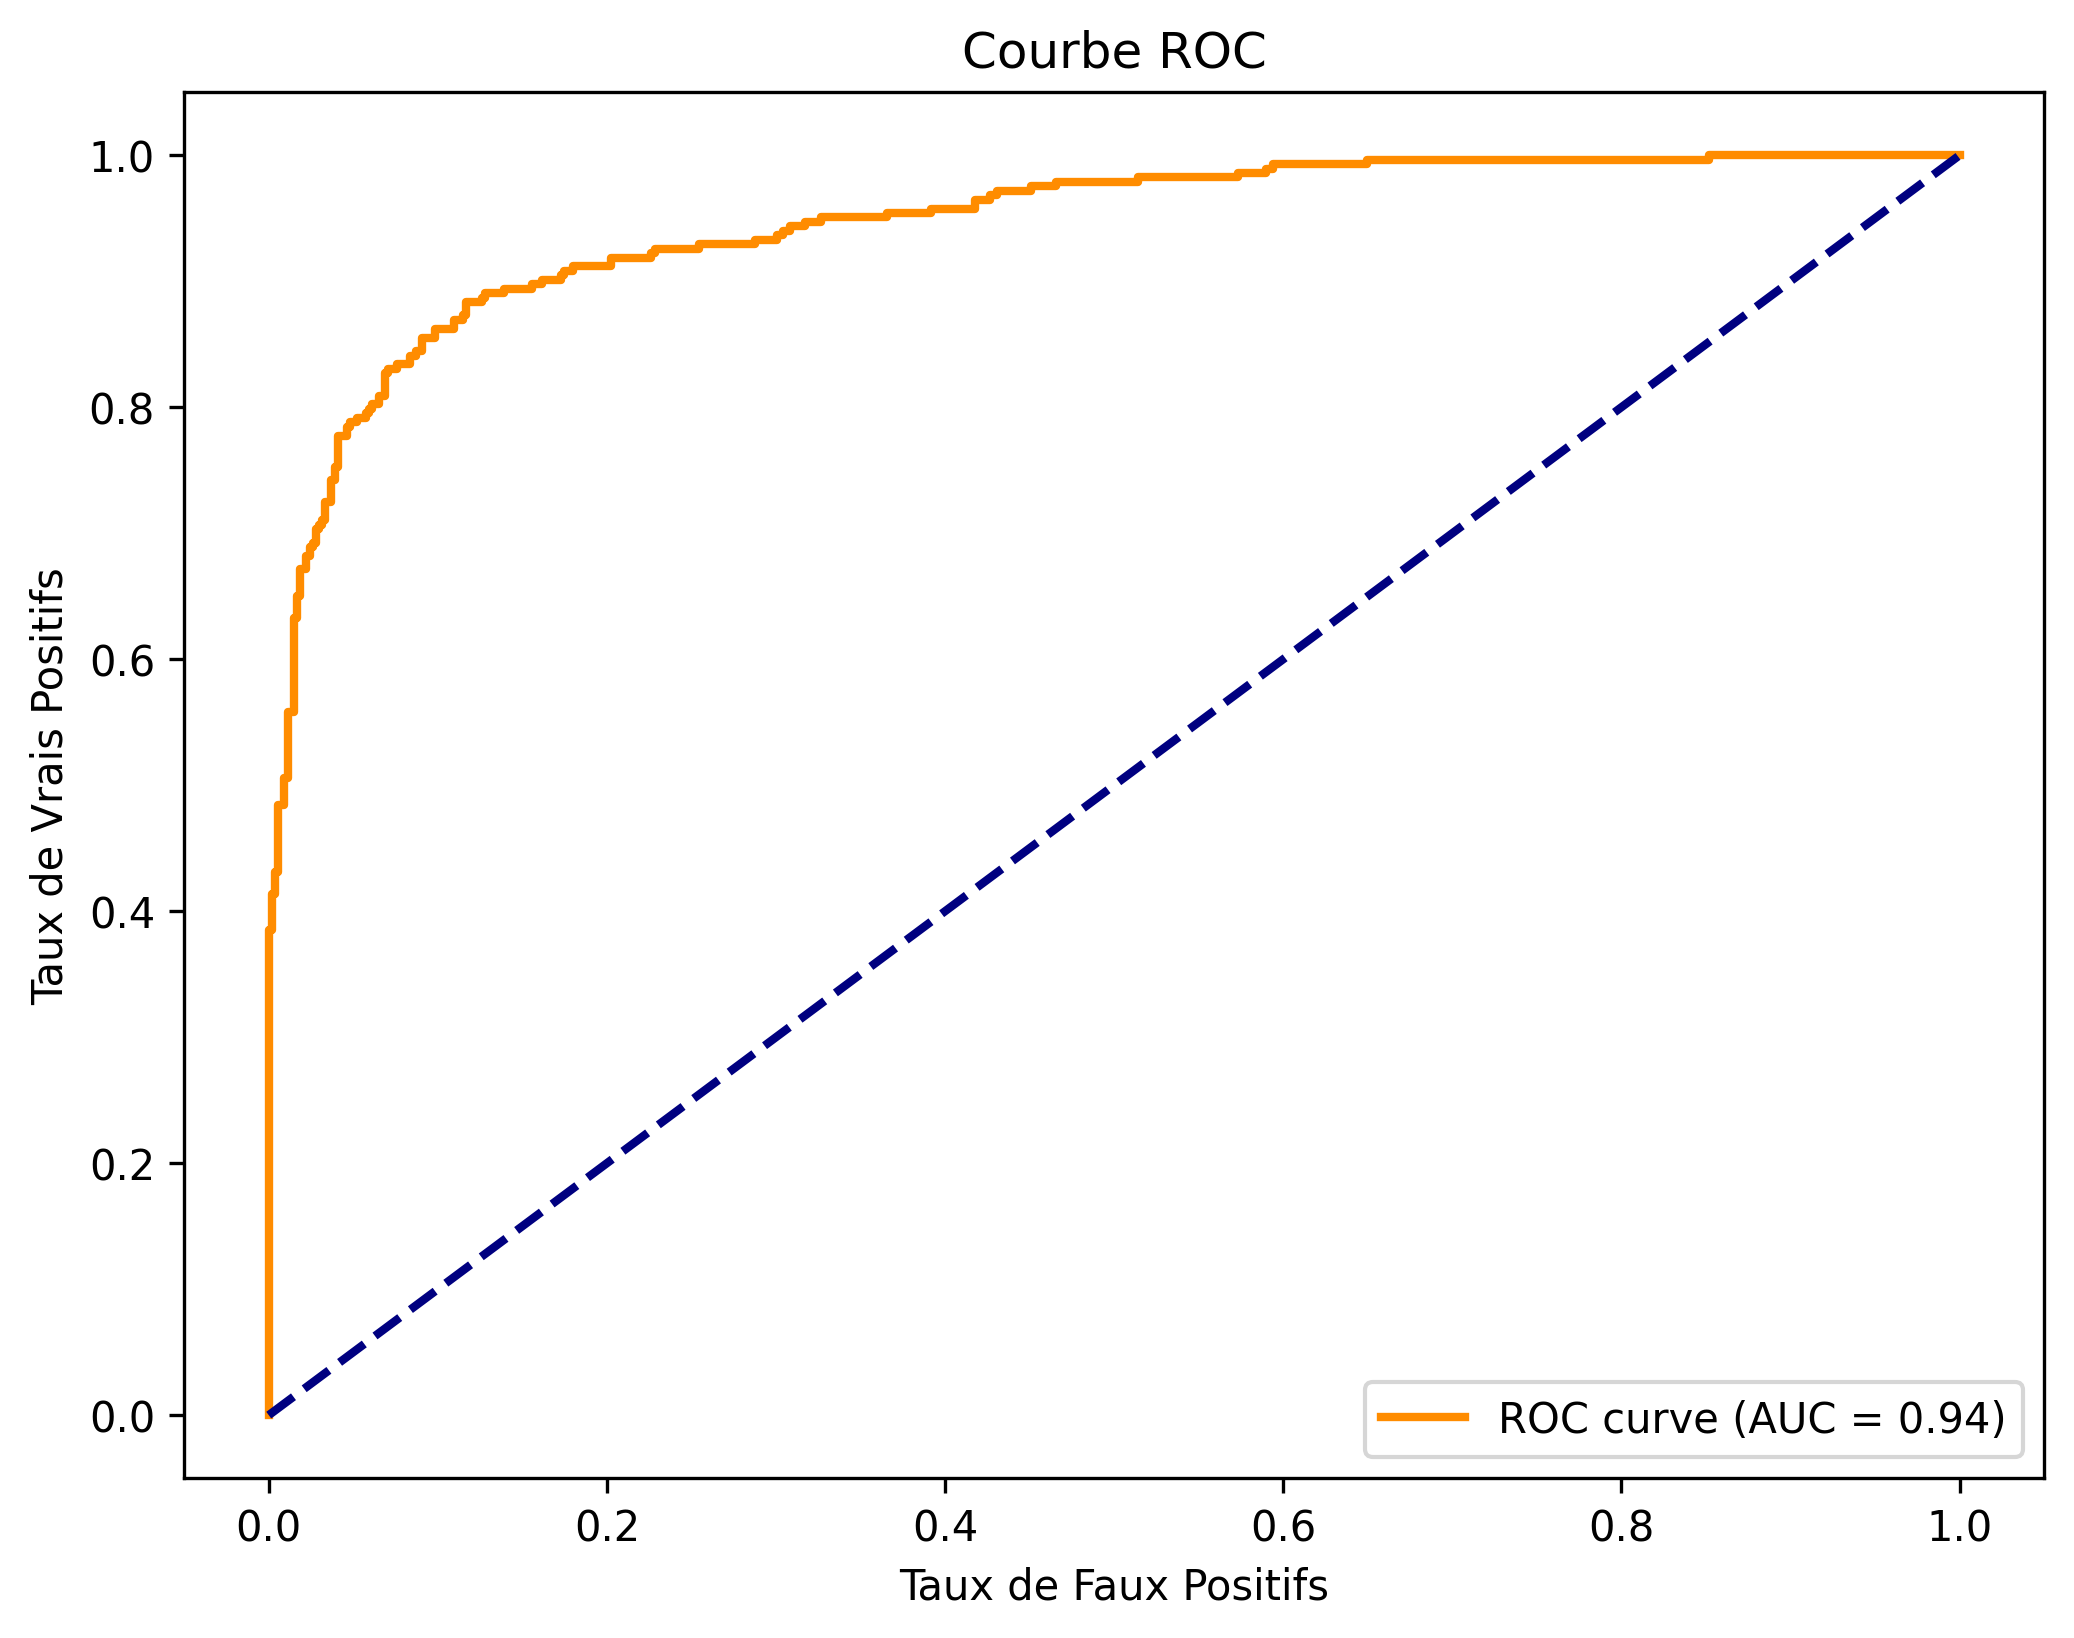
\includegraphics[width=\textwidth]{roc_XGBoost.png}
        \caption{XGBoost (AUC = 0.94)}
    \end{minipage}
    \vspace{0.3cm}
    \begin{minipage}{0.48\textwidth}
        \centering
        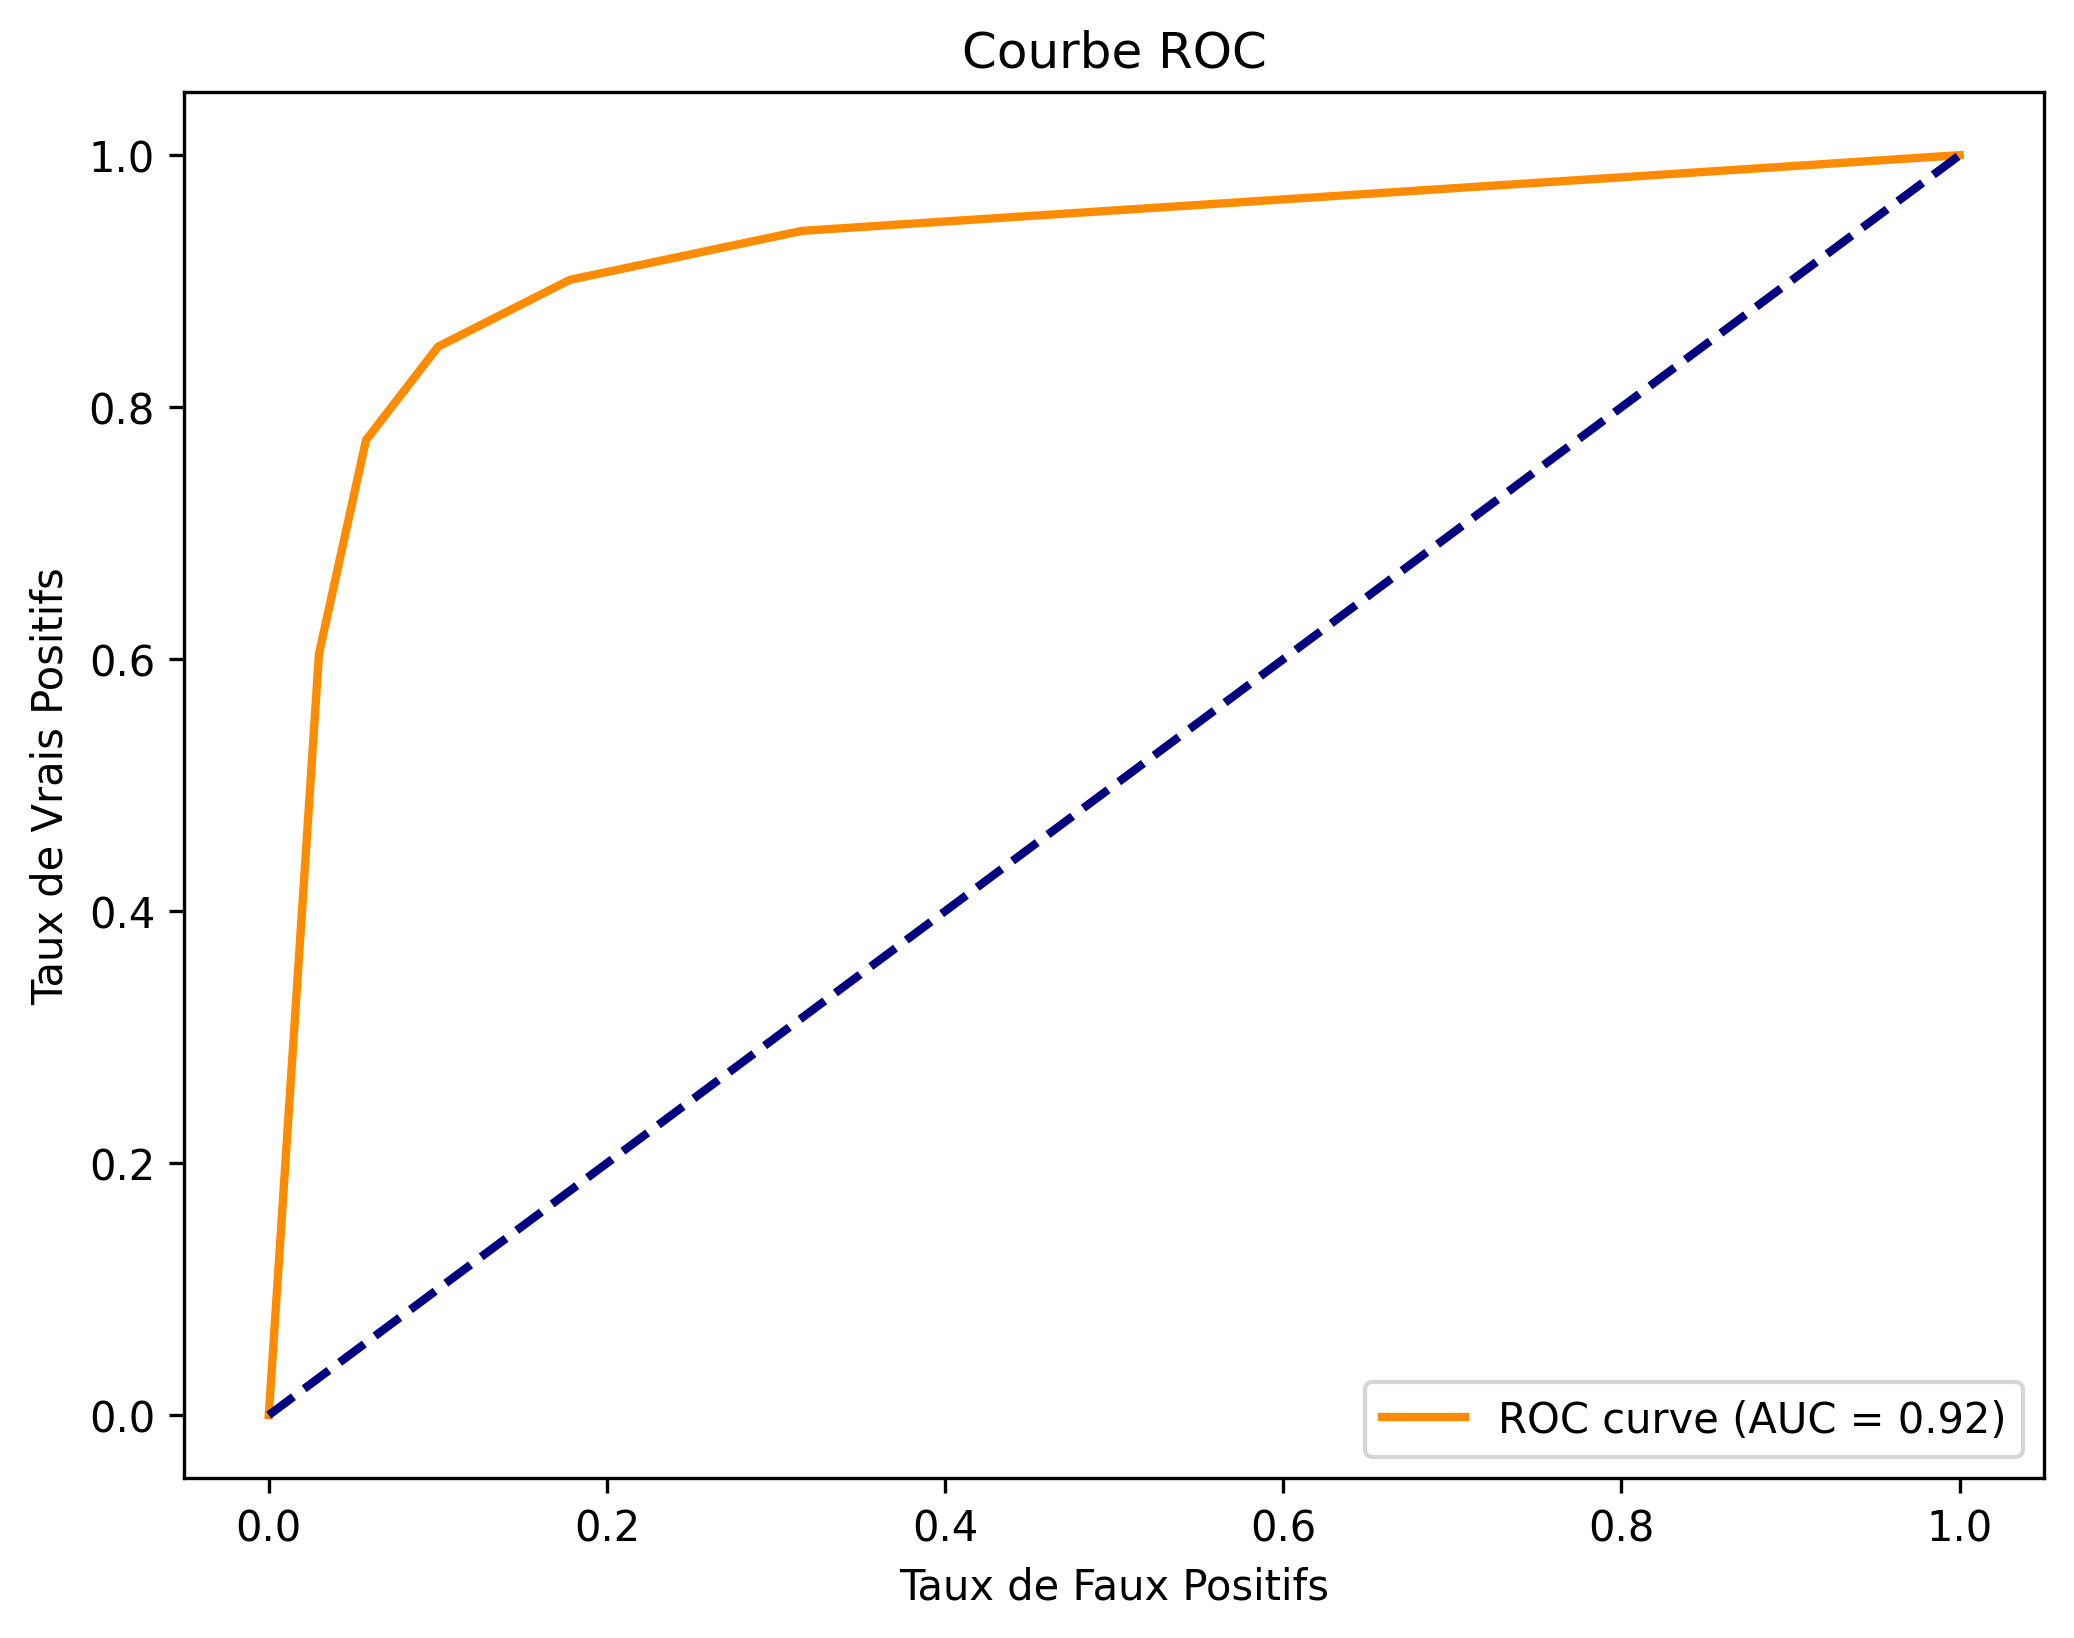
\includegraphics[width=\textwidth]{roc_KNN.png}
        \caption{KNN (AUC = 0.92)}
    \end{minipage}
    \hfill
    \begin{minipage}{0.48\textwidth}
        \centering
        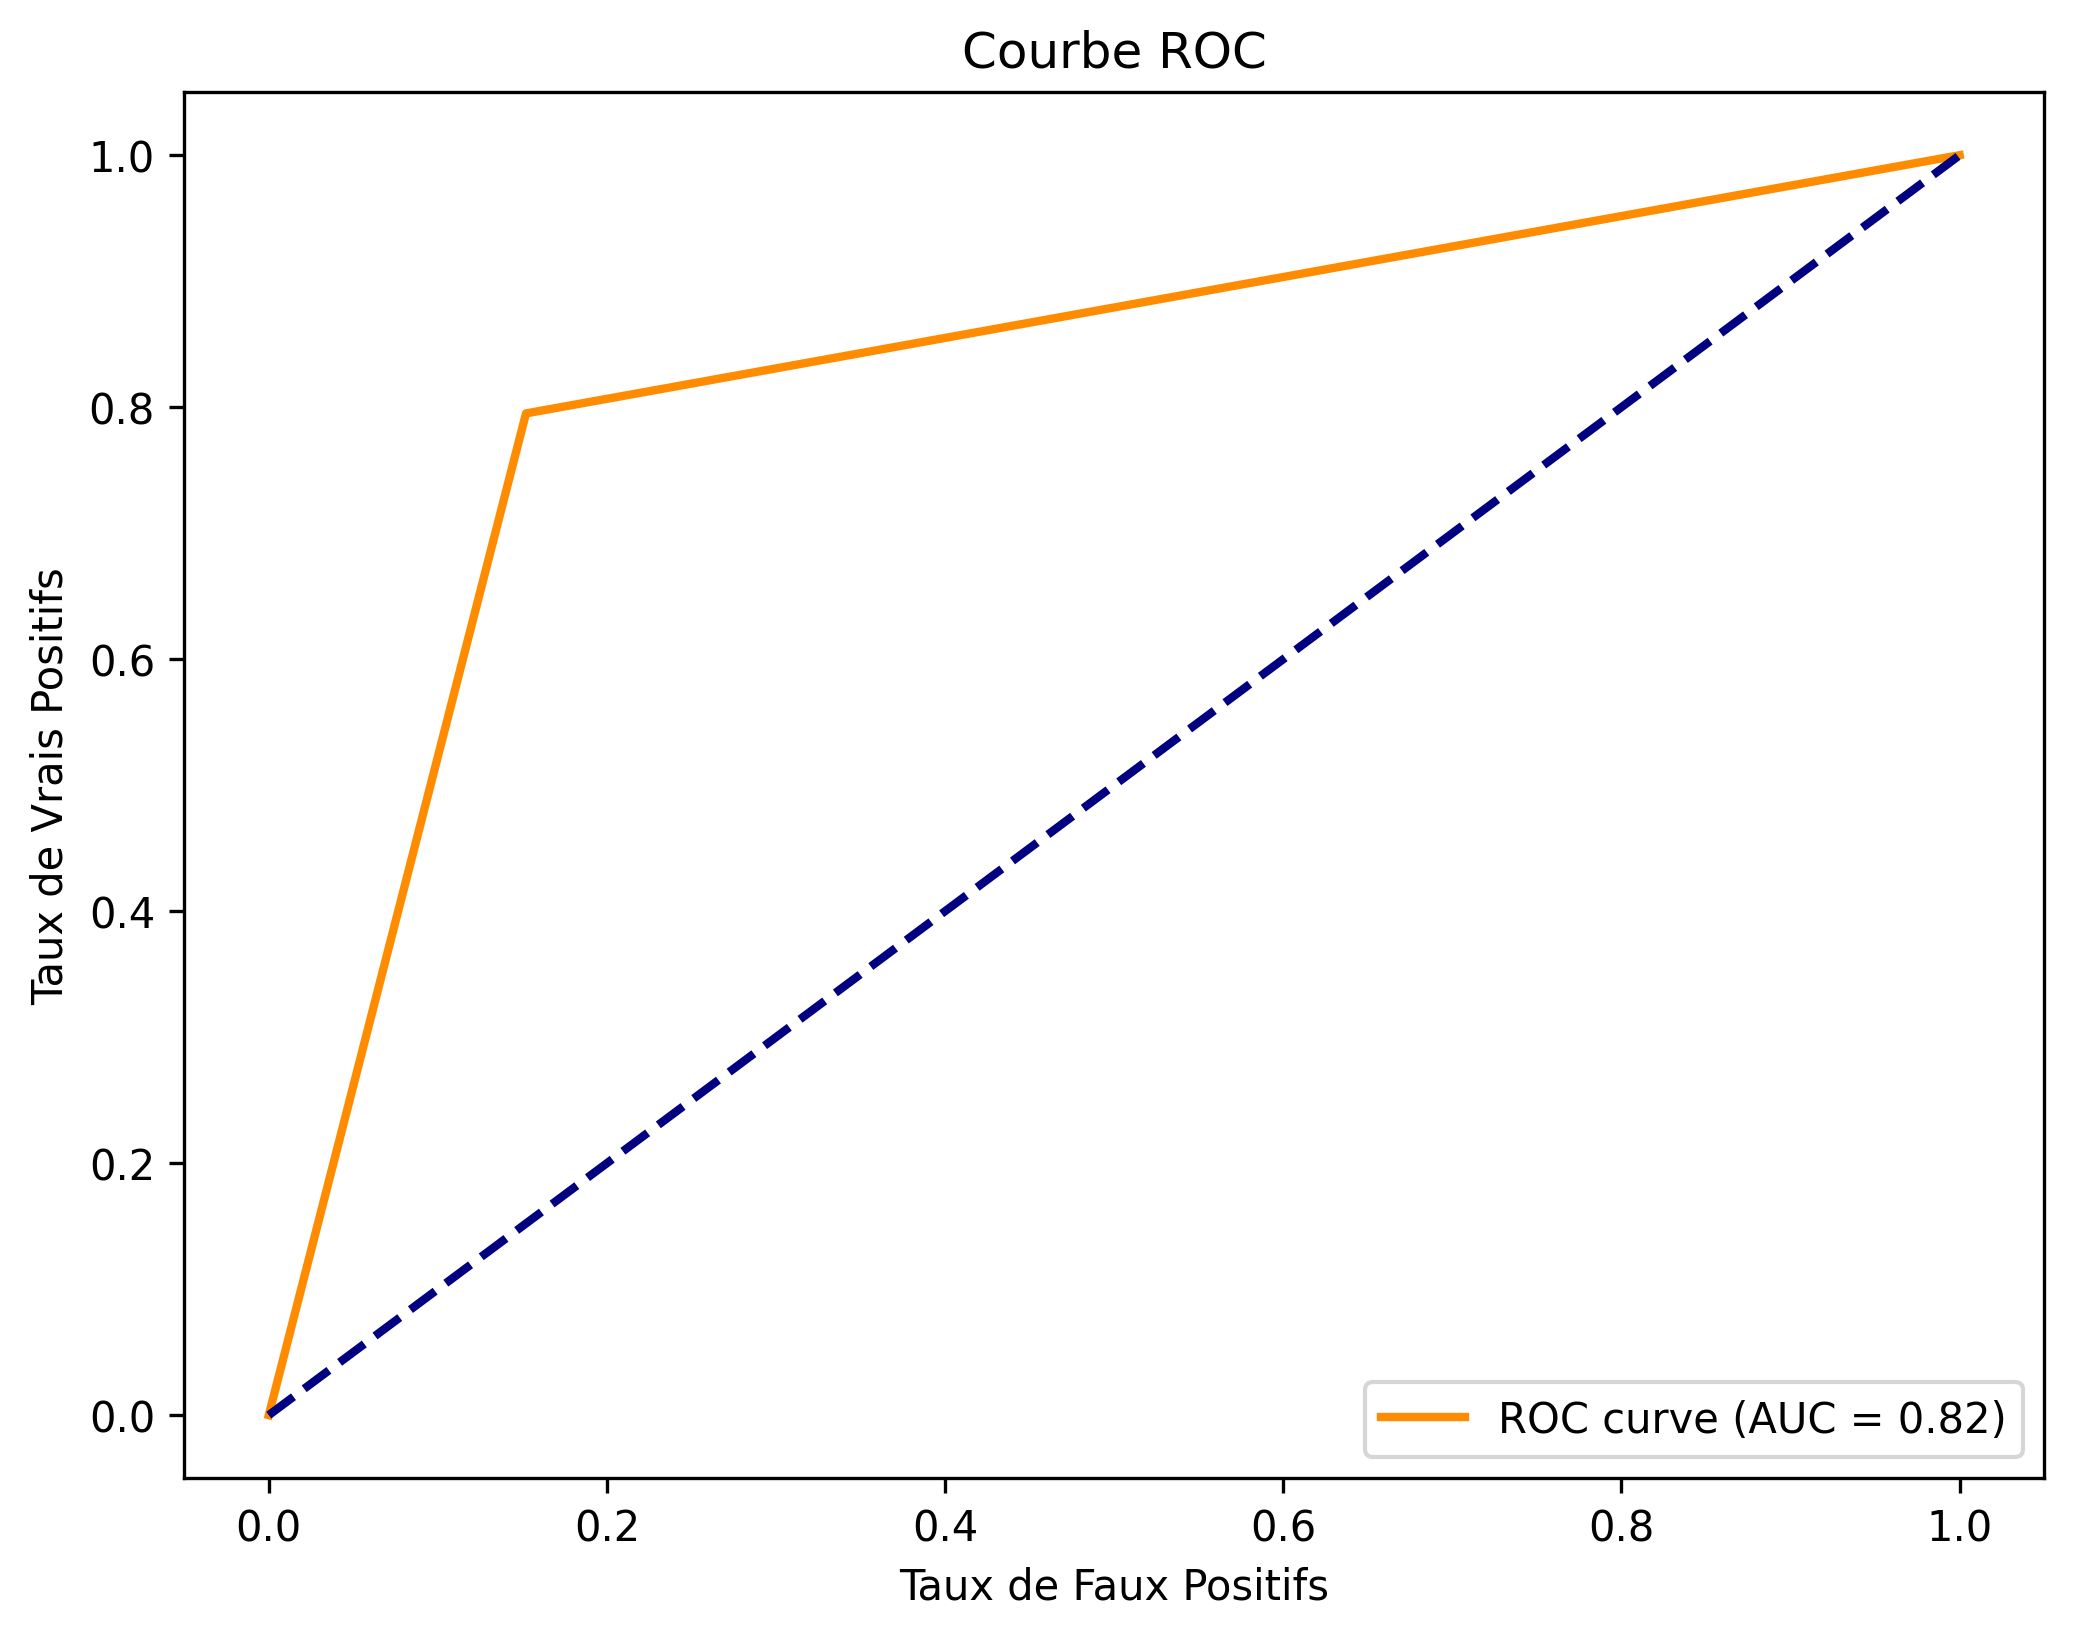
\includegraphics[width=\textwidth]{roc_DecisionTree.png}
        \caption{Decision Tree (AUC = 0.82)}
    \end{minipage}
    \caption{Comparaison des courbes ROC et des scores AUC pour les quatre modèles testés.}
\end{figure}

\textbf{Interprétation :} Bien que le Random Forest et le XGBoost présentent des scores AUC identiques (0.94), le Random Forest a été privilégié pour sa stabilité et sa moindre sensibilité au sur-apprentissage sur notre volume de données. Le Decision Tree présente la performance la plus faible (AUC = 0.82), confirmant l'intérêt d'utiliser des méthodes d'ensemble.

\newpage
\subsubsection{Gestion du déséquilibre par SMOTE}
Pour traiter le déséquilibre des classes (moins de départs que de clients fidèles), nous avons appliqué l'algorithme \textbf{SMOTE} (Synthetic Minority Over-sampling Technique) sur les données d'entraînement. Cela permet au modèle de mieux apprendre les caractéristiques des clients "Churn" sans être biaisé par la majorité.


\subsubsection{Analyse des Matrices de Confusion}
L'examen des matrices de confusion permet de comparer la précision réelle de chaque modèle. Nous observons ici la capacité de chaque algorithme à distinguer les clients fidèles (Classe 0) des clients en situation de Churn (Classe 1).

\begin{figure}[htbp]
    \centering
    % Première ligne
    \begin{minipage}{0.48\textwidth}
        \centering
        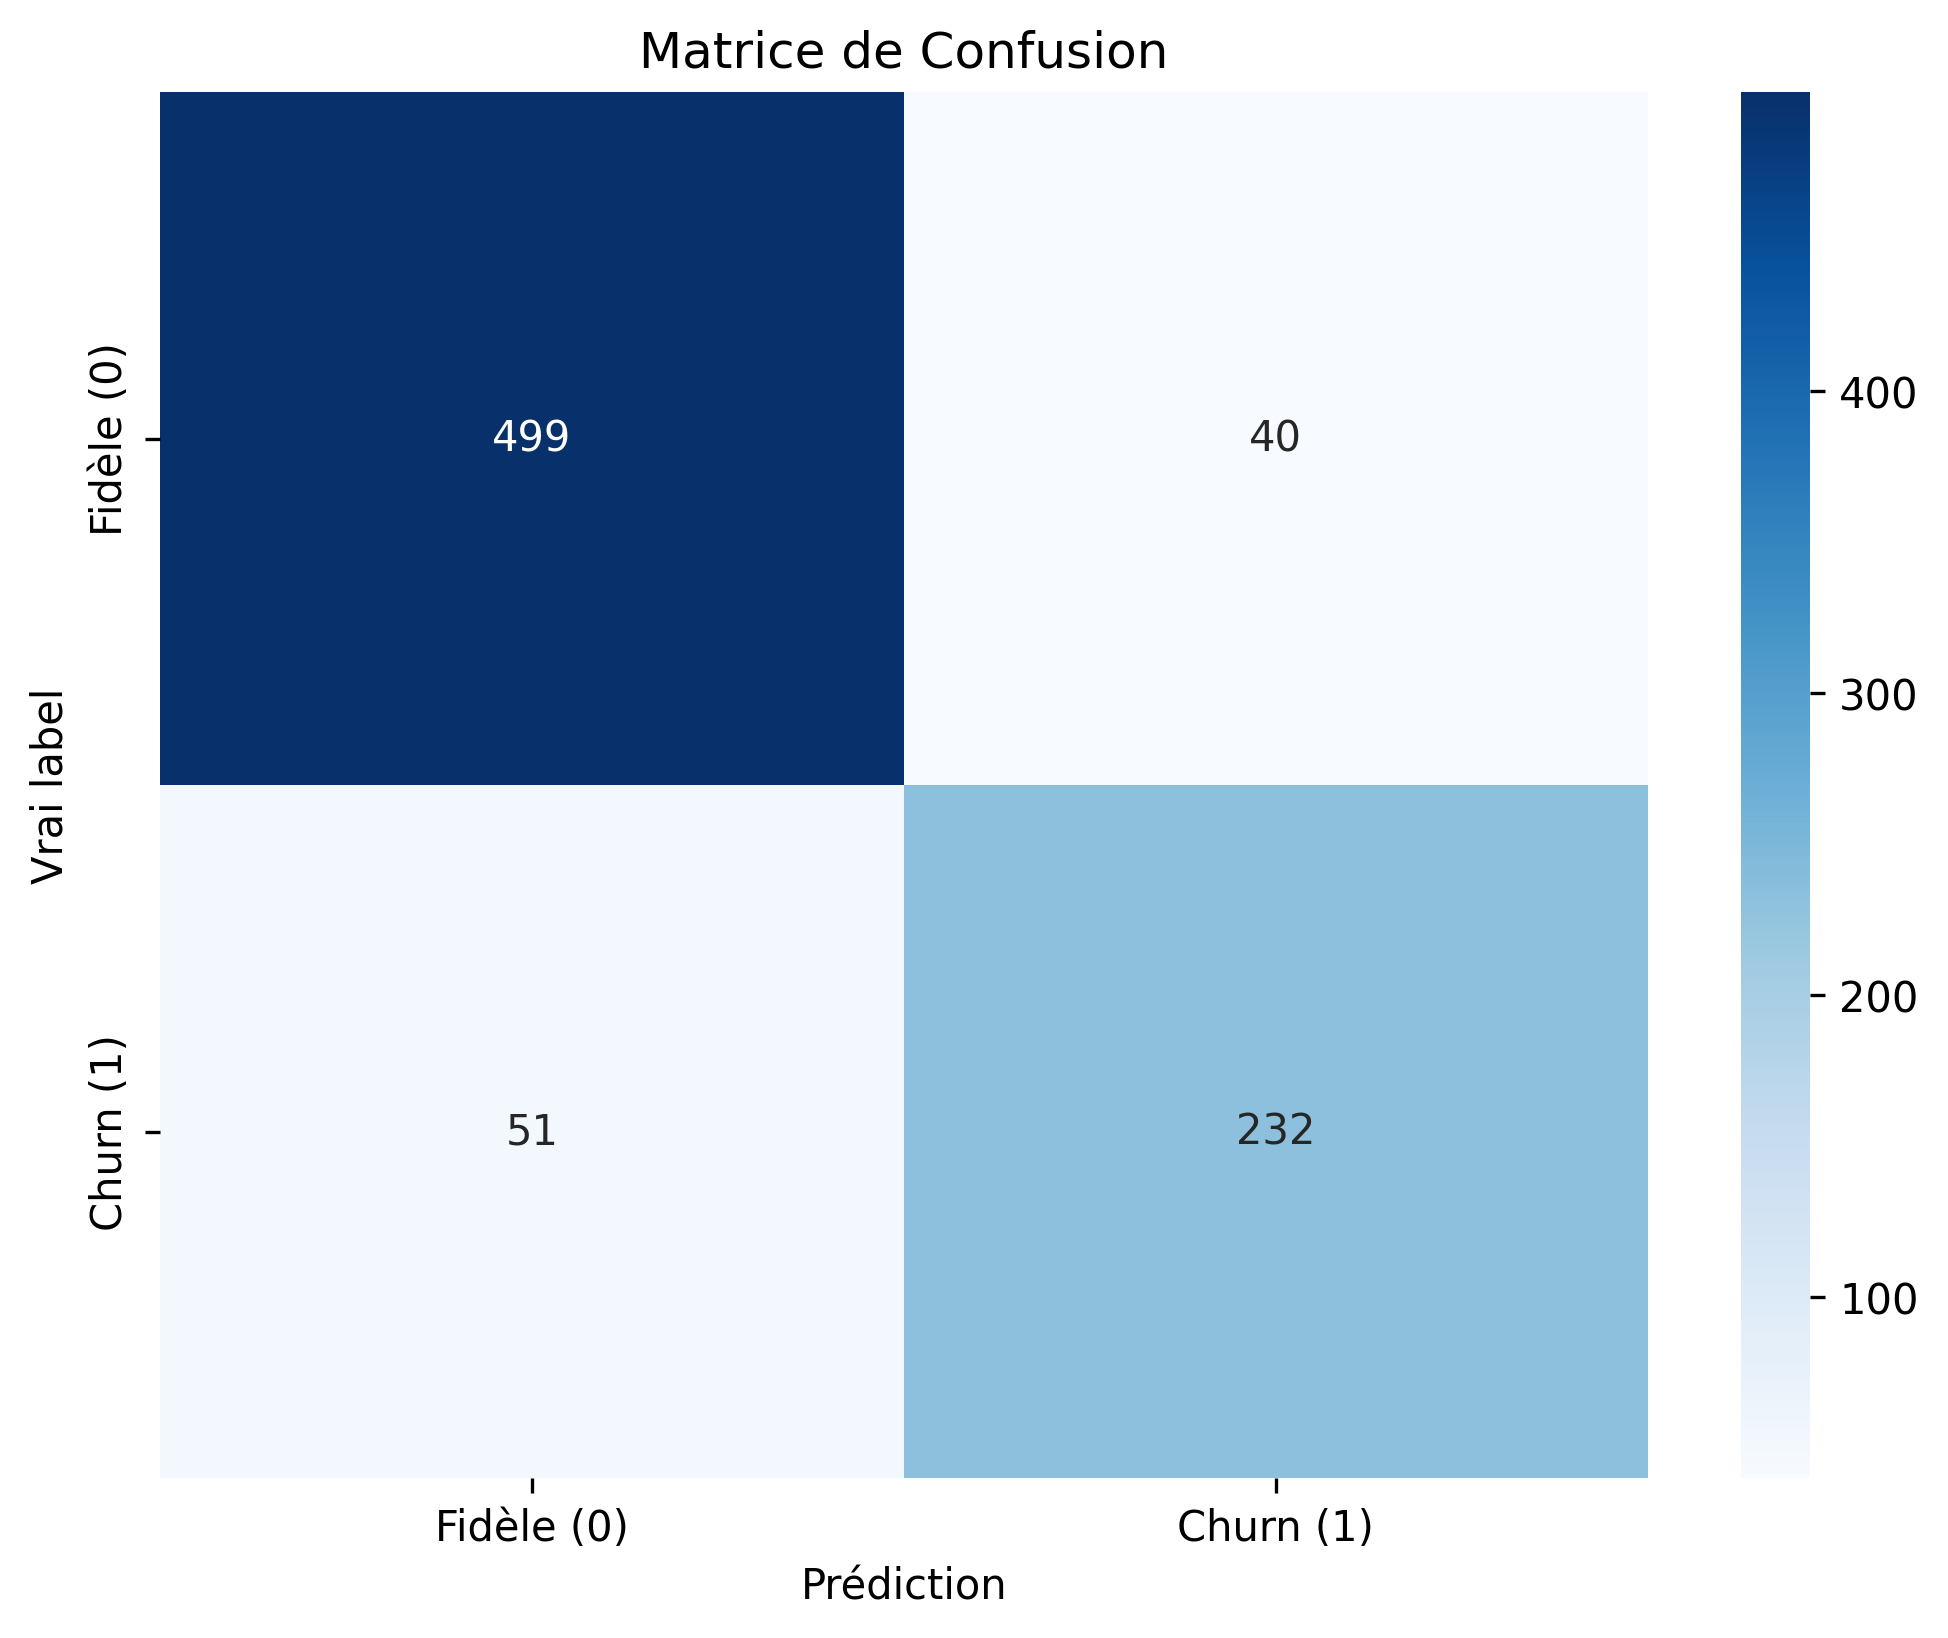
\includegraphics[width=\textwidth]{cm_RandomForest.png}
        \caption{Random Forest}
    \end{minipage}
    \hfill
    \begin{minipage}{0.48\textwidth}
        \centering
        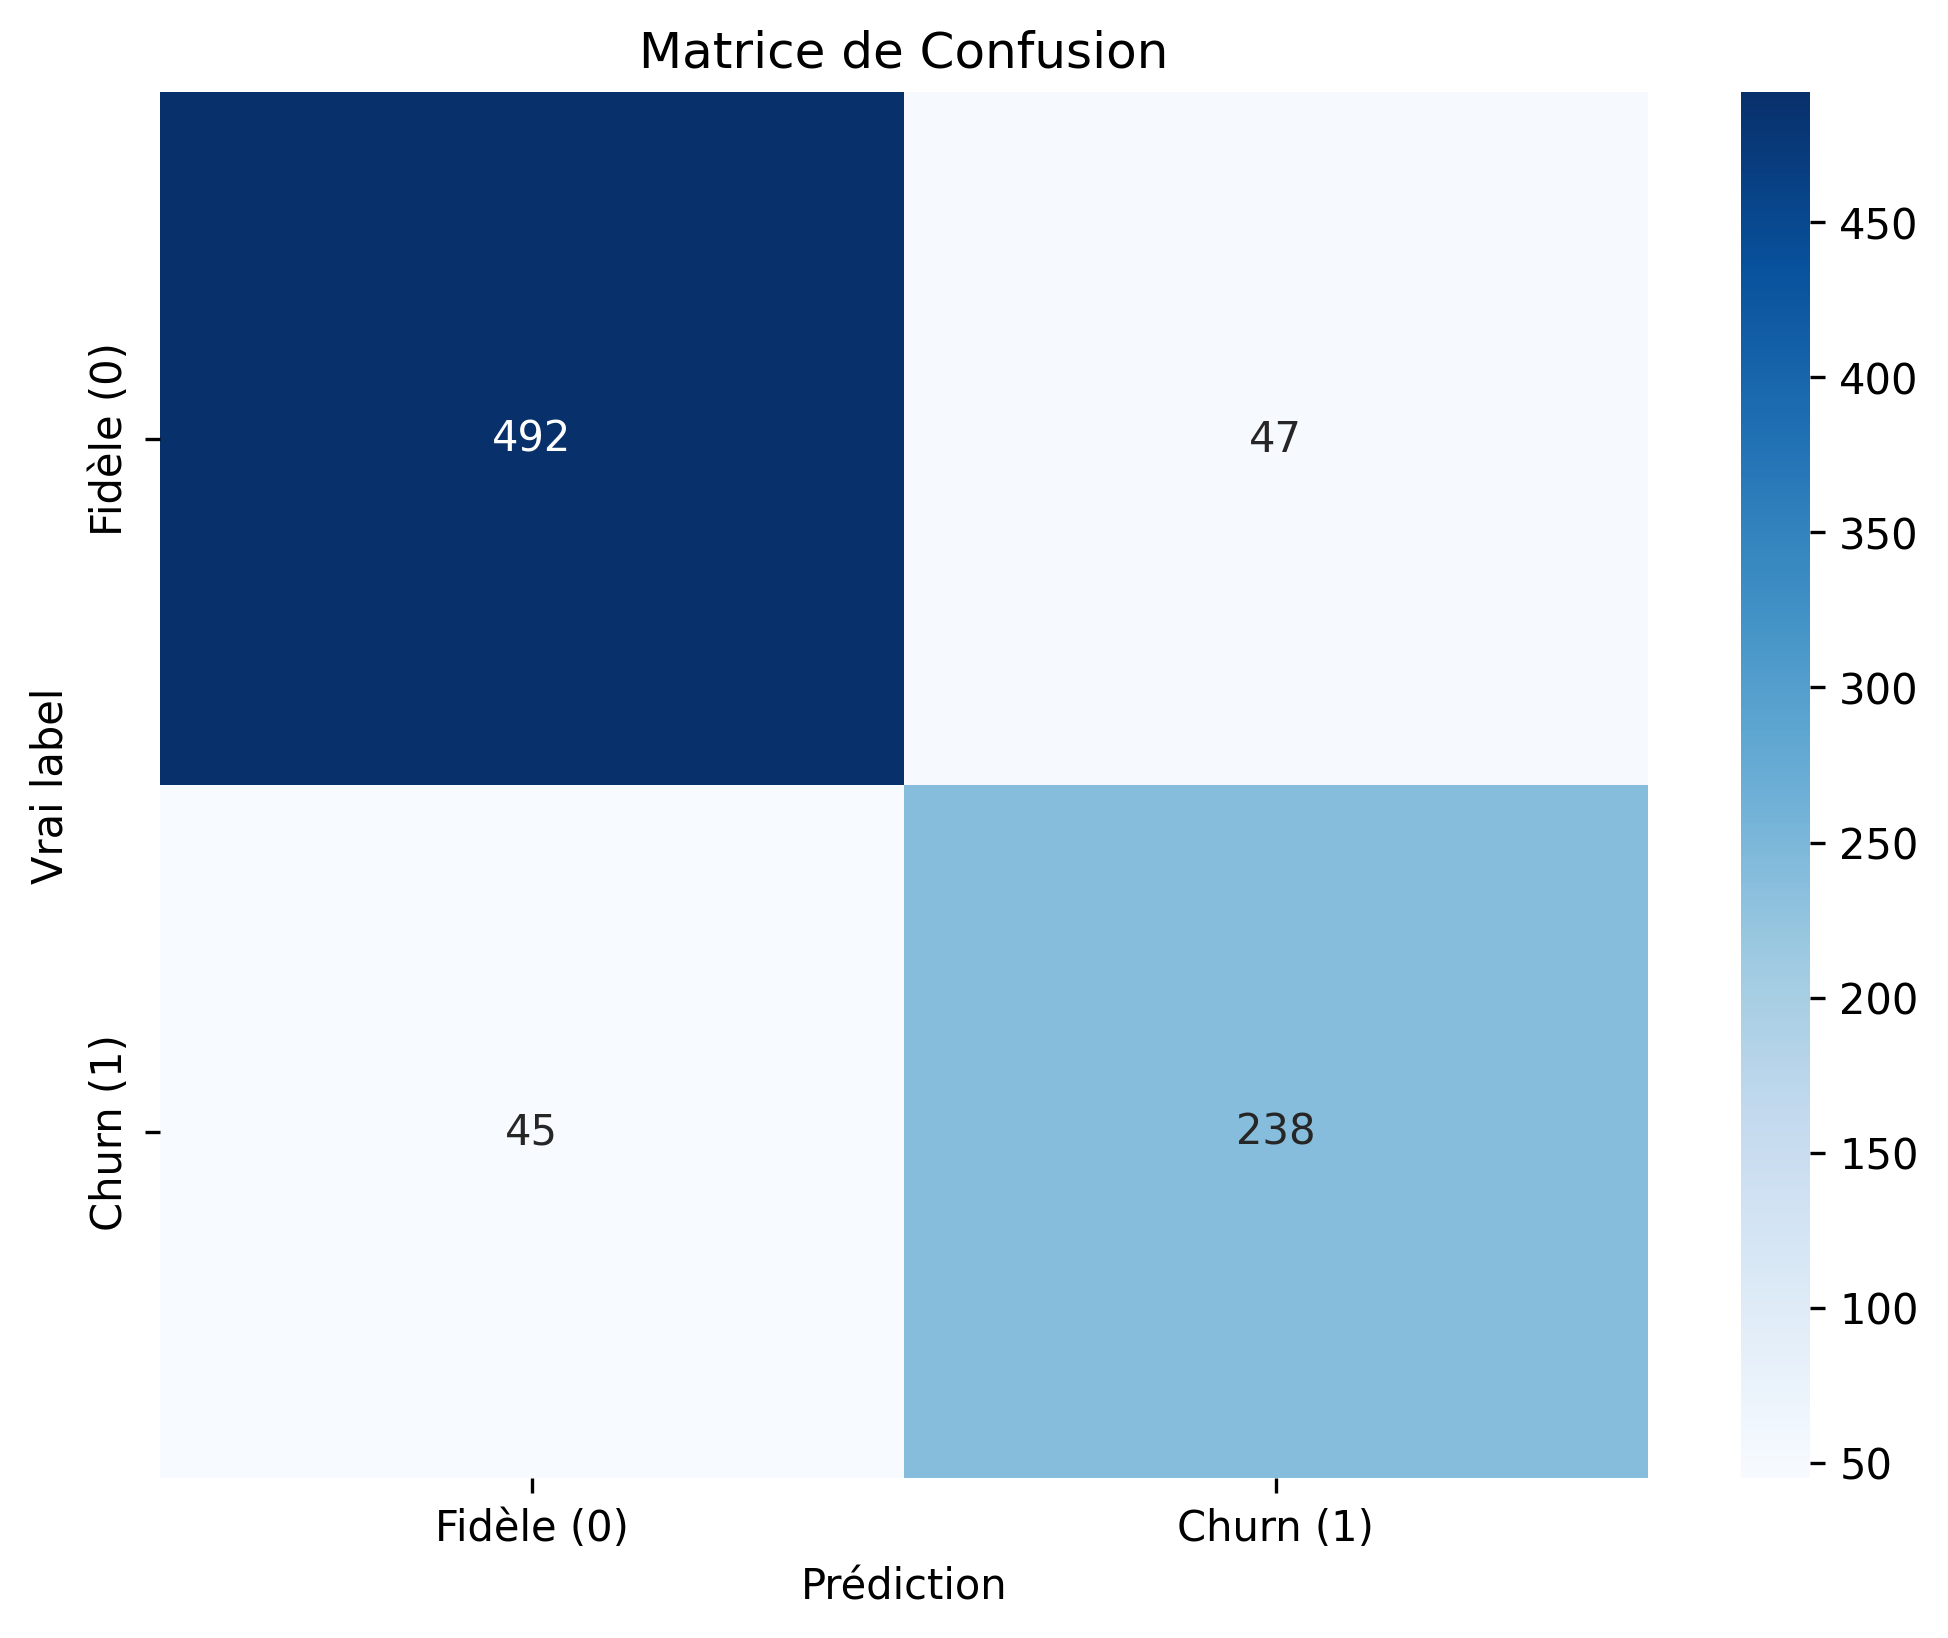
\includegraphics[width=\textwidth]{cm_XGBoost.png}
        \caption{XGBoost}
    \end{minipage}
    
    \vspace{0.5cm} % Espace entre les deux lignes
    
    % Deuxième ligne
    \begin{minipage}{0.48\textwidth}
        \centering
        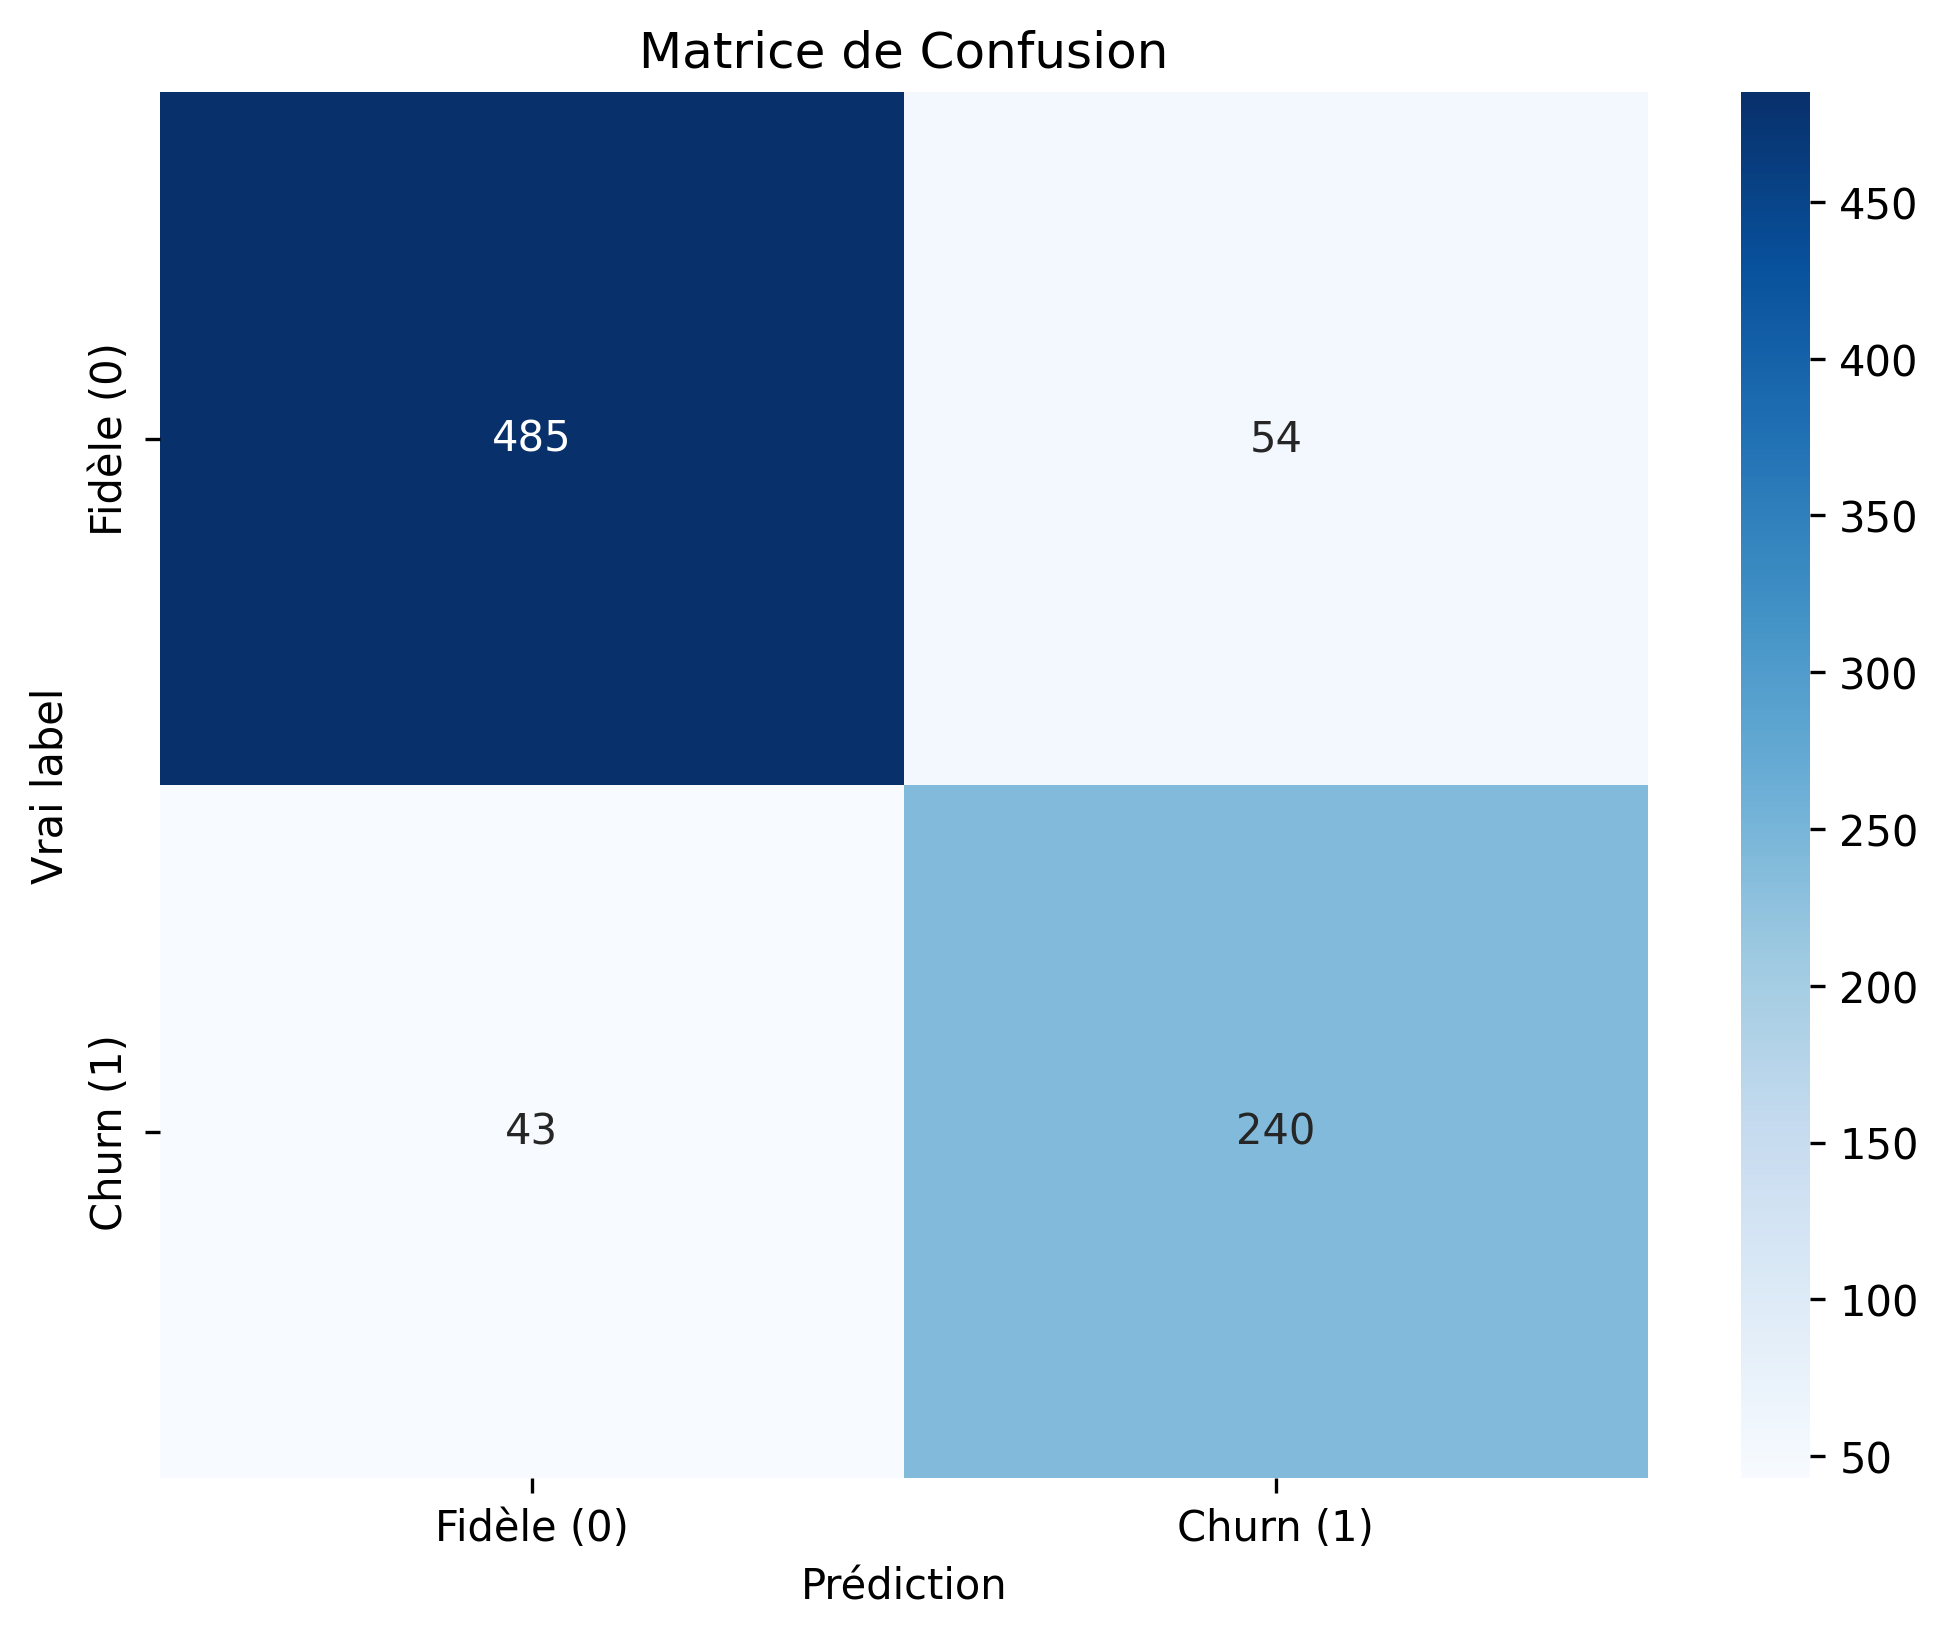
\includegraphics[width=\textwidth]{cm_KNN.png}
        \caption{KNN}
    \end{minipage}
    \hfill
    \begin{minipage}{0.48\textwidth}
        \centering
        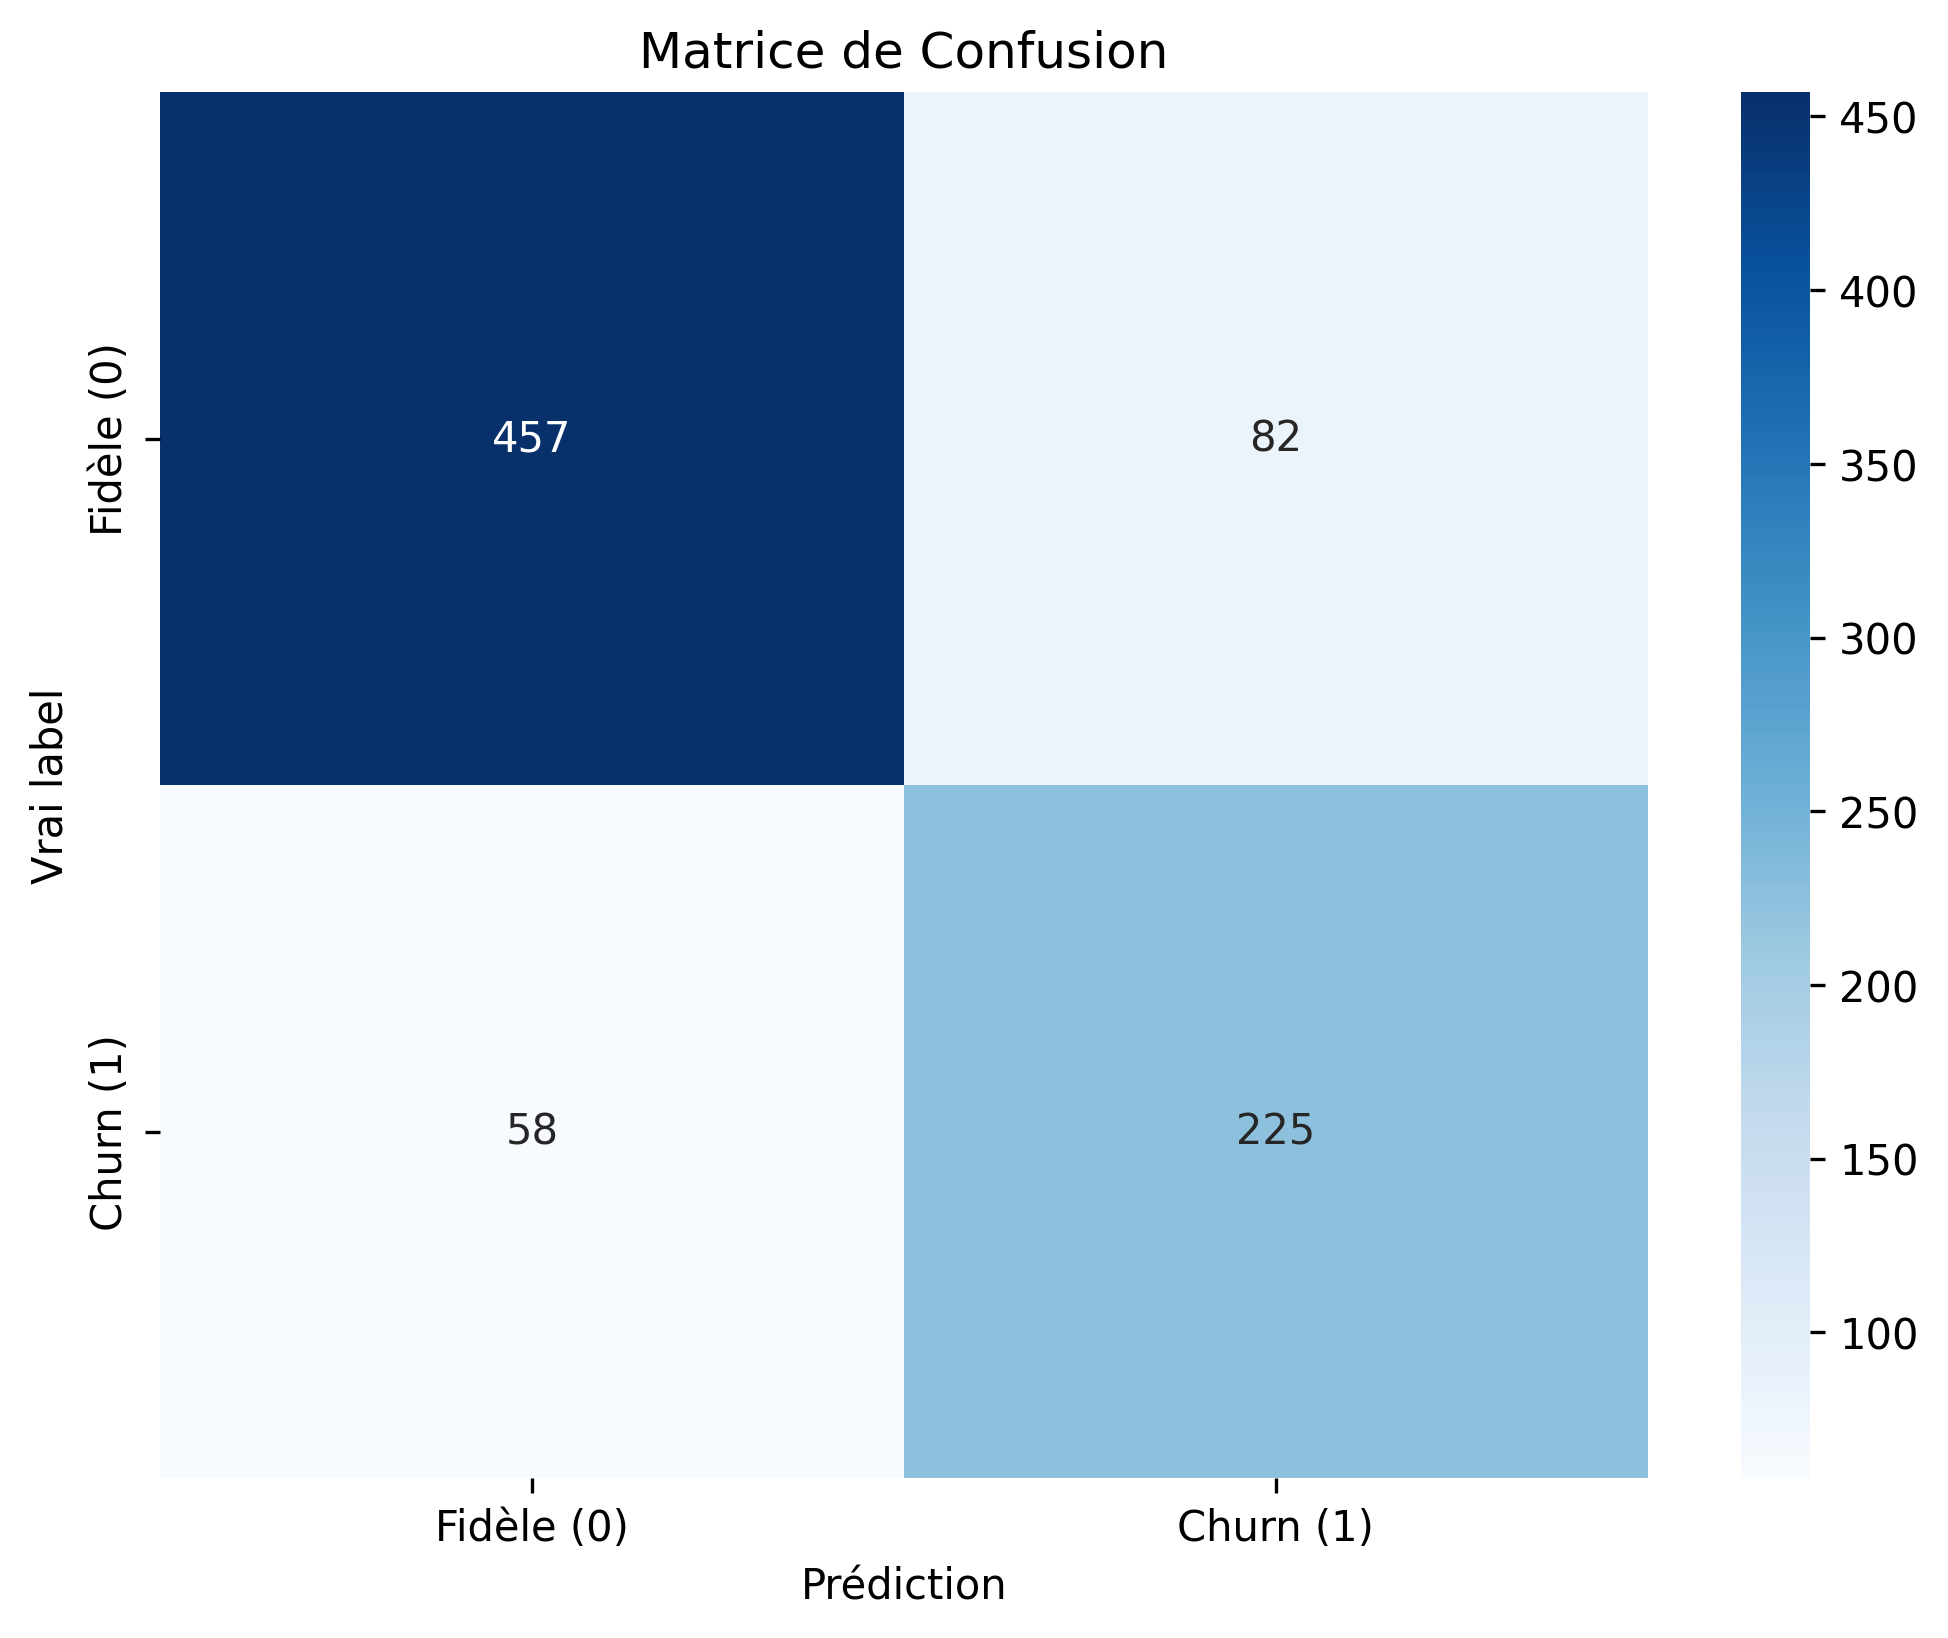
\includegraphics[width=\textwidth]{cm_DecisionTree.png}
        \caption{Decision Tree}
    \end{minipage}
    \caption{Matrices de confusion comparées pour les quatre modèles de classification.}
\end{figure}



\subsubsection{Choix de l'algorithme : Random Forest}
Nous avons privilégié l'algorithme \textbf{Random Forest Classifier} pour cette tâche finale de classification. 

\begin{itemize}
    \item \textbf{Justification :} Contrairement à un arbre de décision simple, la forêt aléatoire réduit le risque de sur-apprentissage en combinant plusieurs arbres (approche par \textit{Bagging}). Comme illustré précédemment dans sa \textbf{matrice de confusion}, le modèle atteint un haut niveau de détection des clients fidèles (499 prédictions correctes) tout en maintenant un très faible taux de faux positifs.
    \item \textbf{Robustesse :} Elle gère nativement les interactions entre les variables complexes, comme la corrélation entre le score de satisfaction et le nombre de tickets de support ouverts.
\end{itemize}

\subsubsection{Métriques d'évaluation : Précision et Rappel}
Le succès du modèle ne se mesure pas uniquement par son exactitude globale (\textit{Accuracy}), mais par sa capacité à équilibrer deux indicateurs critiques :
\begin{itemize}
    \item \textbf{Le Rappel (Recall) :} Crucial dans notre contexte, il mesure la capacité du modèle à détecter \textbf{tous} les clients qui vont réellement partir. Un rappel élevé garantit qu'aucun client "à risque" n'est ignoré par le système.
    \item \textbf{La Précision :} Elle assure que les clients identifiés comme étant en situation de "Churn" le sont réellement, permettant ainsi de cibler les campagnes de rétention de manière efficiente et d'optimiser les coûts marketing.
\end{itemize}


\subsection{Régression des Dépenses (MonetaryTotal)}
En parallèle, nous cherchons à prédire la variable continue \texttt{MonetaryTotal} afin d'estimer la valeur vie client (\textit{Customer Lifetime Value}).

\subsubsection{Approche de régression et Choix Algorithmique}
L'objectif est d'estimer le montant total qu'un client va dépenser. Pour cette tâche, nous avons porté notre choix sur le \textbf{Random Forest Regressor}. 

\begin{itemize}
    \item \textbf{Justification Technique :} Ce choix est motivé par la capacité de cet algorithme à traiter des relations non-linéaires complexes entre les variables. Mathématiquement, le Random Forest Regressor est conçu pour minimiser nativement l'erreur quadratique (\textbf{MSE/RMSE}) lors de sa phase d'apprentissage.
    \item \textbf{Indicateur de référence :} La \textbf{RMSE} (\textit{Root Mean Square Error}) constitue notre métrique de référence conceptuelle. Plus cette valeur est faible, plus la prédiction du montant est proche de la réalité transactionnelle. Bien que l'interface se concentre sur la prédiction directe en Dinars, la réduction de cette erreur est au cœur du processus d'entraînement du modèle.
\end{itemize}


\subsection{Optimisation et Recherche d'Hyperparamètres}
Pour obtenir les meilleures performances possibles, nous ne nous contentons pas des réglages par défaut des algorithmes.

\subsubsection{Utilisation de GridSearchCV et Optuna}
Conformément à la méthodologie du projet, nous avons automatisé la recherche des meilleurs paramètres (comme la profondeur des arbres ou le nombre d'estimateurs) :
\begin{itemize}
    \item \textbf{GridSearchCV :} Permet de tester de manière exhaustive une grille de paramètres prédéfinis via une validation croisée (\textit{Cross-Validation}).
    \item \textbf{Optuna (Alternative avancée) :} Utilise une approche bayésienne pour explorer intelligemment l'espace des paramètres, permettant d'atteindre une convergence plus rapide vers les réglages optimaux.
\end{itemize}



\section{Réalisation et Déploiement}

L'ultime étape de ce projet consiste à rendre les modèles prédictifs accessibles via une interface utilisateur. Cette phase de déploiement transforme nos scripts de recherche en une application opérationnelle.

\subsection{Architecture de la Solution}
Pour garantir la maintenabilité et la robustesse de l'application, nous avons adopté une structure de projet modulaire, conforme aux standards de l'ingénierie logicielle.

\begin{itemize}
    \item \textbf{Dossier \texttt{src/} :} Contient le cœur logique du projet, notamment \texttt{preprocessing.py} pour le nettoyage des données et \texttt{train\_model.py} pour l'entraînement.
    \item \textbf{Dossier \texttt{models/} :} Stocke les objets sérialisés (\texttt{.pkl} ou \texttt{.joblib}) tels que le scaler, le modèle PCA et les modèles de prédiction (Random Forest).
    \item \textbf{Dossier \texttt{app/} :} Regroupe les fichiers liés à l'interface utilisateur développée avec \textbf{Streamlit}, permettant de servir le modèle en temps réel.
\end{itemize}

\subsection{Présentation de l'Interface Streamlit}
Le choix de Streamlit s'explique par sa capacité à transformer des scripts Python en tableaux de bord interactifs sans nécessiter de développement Front-End complexe. L'application propose deux modes d'utilisation :

\subsubsection{Mode Validation par Lot (Batch Processing)}
Ce mode est destiné aux analyses massives. 



\begin{itemize}
    \item \textbf{Fonctionnement :} L'utilisateur télécharge un fichier CSV contenant les données brutes de plusieurs clients.
    \item \textbf{Traitement :} L'application applique automatiquement le pipeline de prétraitement et renvoie un fichier complet incluant les prédictions de Churn et les segments attribués pour chaque client.
\end{itemize}

\begin{figure}[htbp]
    \centering
    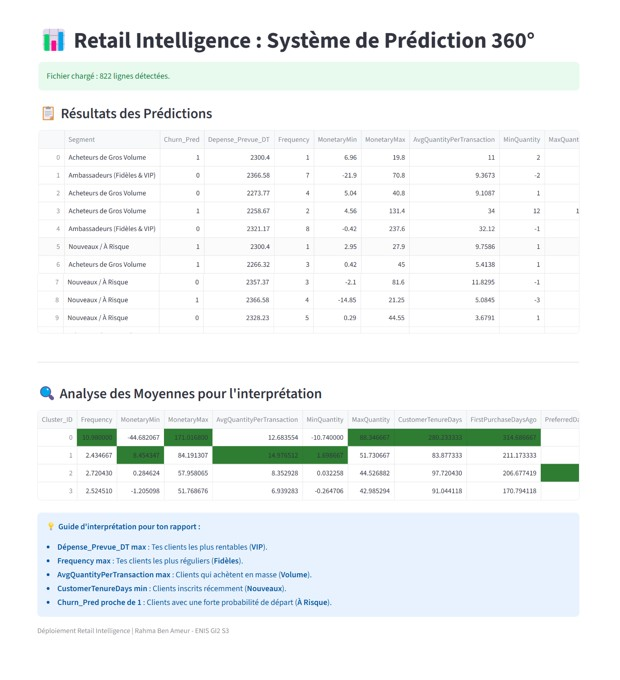
\includegraphics[width=0.85\textwidth]{capture_web2.jpg} 
    \caption{Interface du mode de traitement par lot (Upload de fichier CSV).}
\end{figure}
\newpage

\subsubsection{Mode Analyse Individuelle}
Ce mode permet une évaluation granulaire en temps réel via un formulaire dynamique.


\begin{itemize}
    \item \textbf{Interaction :} L'utilisateur saisit manuellement les caractéristiques d'un client (âge, région, score de satisfaction, etc.).
    \item \textbf{Réactivité :} Le modèle calcule instantanément la probabilité de départ et le profil du client, offrant une aide à la décision immédiate pour un conseiller clientèle.
\end{itemize}

\begin{tcolorbox}[title=Rigueur du Pipeline Applicatif]
\begin{itemize}
    \item \textbf{Robustesse :} L'interface traite l'intégralité des \textbf{40 variables features}, garantissant que la prédiction repose sur l'ensemble du contexte client. 
    \item \textbf{Automatisation :} Elle inclut un encodage automatique des 13 colonnes textuelles (via \texttt{Categorical.codes}) et une imputation des valeurs manquantes avant la projection PCA, rendant l'outil accessible à des utilisateurs non-techniciens.
\end{itemize}
\end{tcolorbox}

\begin{figure}[htbp]
    \centering
    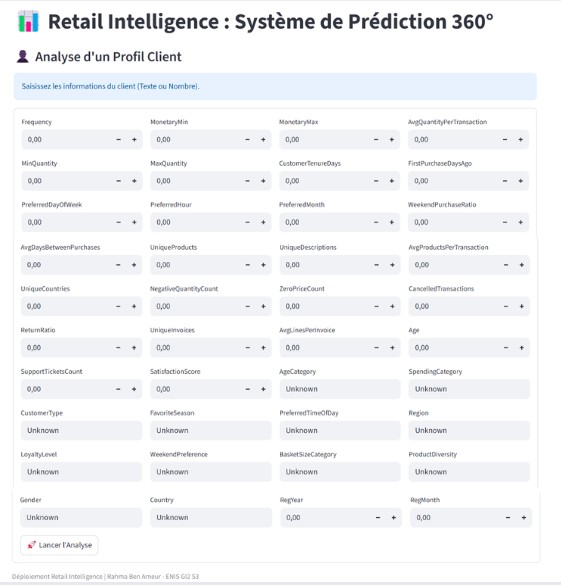
\includegraphics[width=0.85\textwidth]{capture_web1.jpg} 
    \caption{Interface de saisie individuelle pour une prédiction en temps réel.}
\end{figure}


\subsection{Guide d'Utilisation et Déploiement}
Pour assurer la portabilité de la solution sur différentes machines, une procédure d'installation stricte a été définie.

\subsubsection{Gestion des dépendances (\texttt{requirements.txt})}
Toutes les bibliothèques nécessaires (\textit{Scikit-Learn, Pandas, Streamlit, Joblib}) sont répertoriées dans le fichier \texttt{requirements.txt}. L'installation est automatisée via la commande :
\begin{lstlisting}[language=bash]
pip install -r requirements.txt
\end{lstlisting}

\subsubsection{Exécution de l'application}
Le lancement de la plateforme s'effectue simplement en ligne de commande depuis la racine du projet, garantissant une mise en service rapide :
\begin{lstlisting}[language=bash]
streamlit run app/app.py
\end{lstlisting}


\section*{Conclusion Générale et Perspectives}
\addcontentsline{toc}{section}{Conclusion Générale et Perspectives}

Ce projet d'analyse comportementale de la clientèle retail a permis de couvrir l'intégralité du pipeline de la Data Science, de l'exploration brute à la mise en production d'une solution interactive.

\subsection*{Synthèse des Résultats}
Le travail réalisé a abouti à plusieurs résultats concrets :
\begin{itemize}
    \item \textbf{Optimisation de la donnée :} Le passage de 52 variables à 10 composantes principales via la \textbf{PCA} a permis de conserver plus de 85\% de l'information tout en éliminant la redondance statistique.
    \item \textbf{Segmentation Actionnable :} L'algorithme \textbf{K-Means} ($K=4$) a identifié des groupes de clients aux comportements distincts (Ambassadeurs, Clients à Risque, etc.), offrant ainsi une base solide pour des campagnes marketing ciblées.
    \item \textbf{Performance Prédictive :} Le modèle de classification \textbf{Random Forest} a démontré une capacité robuste à anticiper le \textit{Churn}, avec un équilibre optimal entre précision et rappel après optimisation des hyperparamètres.
\end{itemize}

\subsection*{Limites du Modèle}
Malgré la pertinence des résultats, le système actuel présente certaines limites intrinsèques :
\begin{itemize}
    \item \textbf{Staticité des données :} Le modèle repose sur un export CSV "figé". Dans un environnement de production réel, le comportement client évolue quotidiennement, nécessitant une ré-ingestion de données en temps réel (\textit{Streaming}).
    \item \textbf{Biais de l'historique :} Les prédictions sont basées sur le passé. Des événements exceptionnels (soldes agressives, crises économiques) pourraient fausser les résultats si le modèle n'est pas ré-entraîné fréquemment.
\end{itemize}

\subsection*{Perspectives d'Évolution}
Pour transformer ce prototype en un outil industriel de premier plan, plusieurs axes de développement sont envisageables :
\begin{enumerate}
    \item \textbf{Système de Recommandation :} Intégrer un moteur de recommandation de produits (filtrage collaboratif) pour suggérer le prochain achat idéal en fonction du segment du client.
    \item \textbf{Architecture Cloud :} Déployer l'interface Streamlit sur une infrastructure Cloud (AWS ou Google Cloud Platform) pour garantir une haute disponibilité et l'évolutivité de la solution.
    \item \textbf{Deep Learning :} Explorer des architectures de réseaux de neurones récurrents (LSTM) pour analyser les séquences temporelles des achats, au-delà de la simple récence.
\end{enumerate}

\vspace{1cm}
En conclusion, ce projet démontre que l'alliance entre l'ingénierie des données et le machine learning permet de transformer des volumes massifs de transactions en une intelligence stratégique pour l'entreprise.




\end{document}